\RequirePackage[hyphens]{url}
\documentclass[aspectratio=169]{beamer}
\usefonttheme{professionalfonts}
\usepackage[normalem]{ulem}
\usepackage{listings}
\usepackage{transparent}
\usepackage{graphicx}
\graphicspath{ {./img/} }
\usepackage{fnpct}
\usepackage{xcolor}
\usepackage{colortbl}
\usepackage{tikz}
\definecolor{commentsColor}{rgb}{0.497495, 0.497587, 0.497464}
\definecolor{keywordsColor}{rgb}{0.400000, 0.400000, 1.0}
\definecolor{stringColor}{rgb}{1.0, 0.4, 0.4}
\hypersetup{
pdftitle={},
pdfsubject={},
pdfauthor={},
pdfkeywords={HomeTec Pro, CFA3000, CFF3000, AES, PIC18LF45K80, PIC16F1829, MRF89XA, TBLRD}
}

\setbeamertemplate{navigation symbols}{}
\setbeamercolor{frametitle}{fg=white}
\setbeamercolor{background canvas}{bg=black}
\setbeamercolor{normal text}{fg=white}

\usepackage{fontspec}
\newfontfamily\MonaSansBold{Mona Sans Bold}
\setbeamerfont{frametitle}{family=\MonaSansBold}
\setbeamerfont{title}{family=\MonaSansBold}
\setsansfont{Mona Sans}

\title[PIC (un)lock(ed)]{Unlocked: PICing a wireless door access system}

\author[S. Reichel]{Sebastian Reichel}
\date{29.12.2023}

\begin{document}

\begin{frame}
	\begin{columns}
		\begin{column}{0.25\textwidth}
			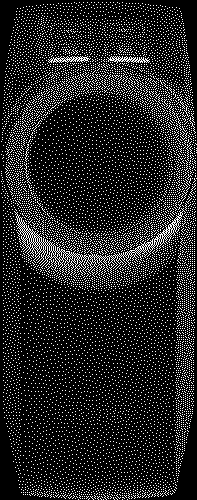
\includegraphics[height=0.9\textheight]{cfa3000-mediumdither.png}
		\end{column}
		\begin{column}{0.75\textwidth}
			
\includegraphics[width=1.0\textwidth]{unlocked.pdf}\\
			\vspace{0.3cm}
			\resizebox{\textwidth}{!}{{\Large \textbf{PICing a wireless door access system}}}
			~\\
			Sebastian Reichel\\
			2023-12-29\\

			\begin{tikzpicture}[remember picture,overlay]
				\node[xshift=-2.5cm,yshift=0.8cm] at (current page.south east){%
				
\includegraphics[width=4cm]{37c3.pdf}};
			\end{tikzpicture}
		\end{column}
	\end{columns}
\end{frame}

\section{Introduction}

\begin{frame}
	\frametitle{\$ whoami}

	\begin{columns}
		\begin{column}{0.7\textwidth}
			\begin{itemize}
				\item Sebastian Reichel
					\begin{itemize}
						\item Deputy lead for fire department diver squad
						\item Part of CERT
						\item Linux kernel engineer at Collabora
						\item Hackspace Oldenburg co-founder
					\end{itemize}
			\end{itemize}
		\end{column}
		\begin{column}{0.3\textwidth}
			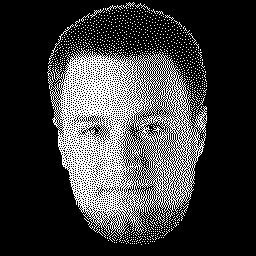
\includegraphics[width=1.0\textwidth]{sre.dithered.png}
		\end{column}
	\end{columns}
\end{frame}

\begin{frame}
	\frametitle{In the beginning there was CFA1000...}

	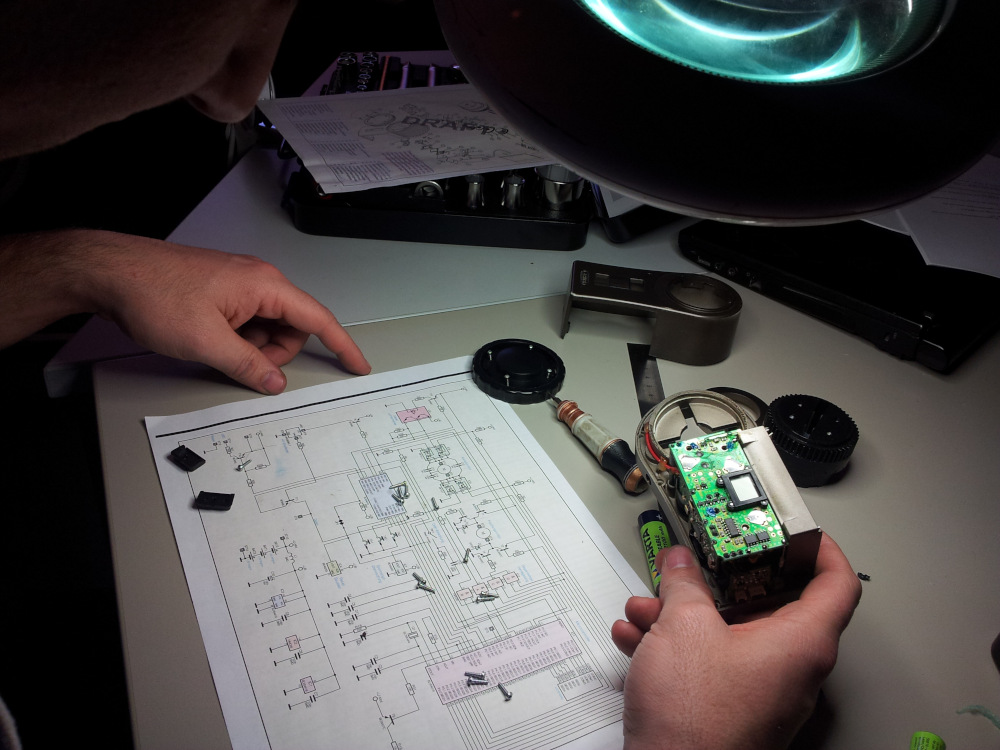
\includegraphics[height=0.75\textheight]{CFA1000-1.jpg}
	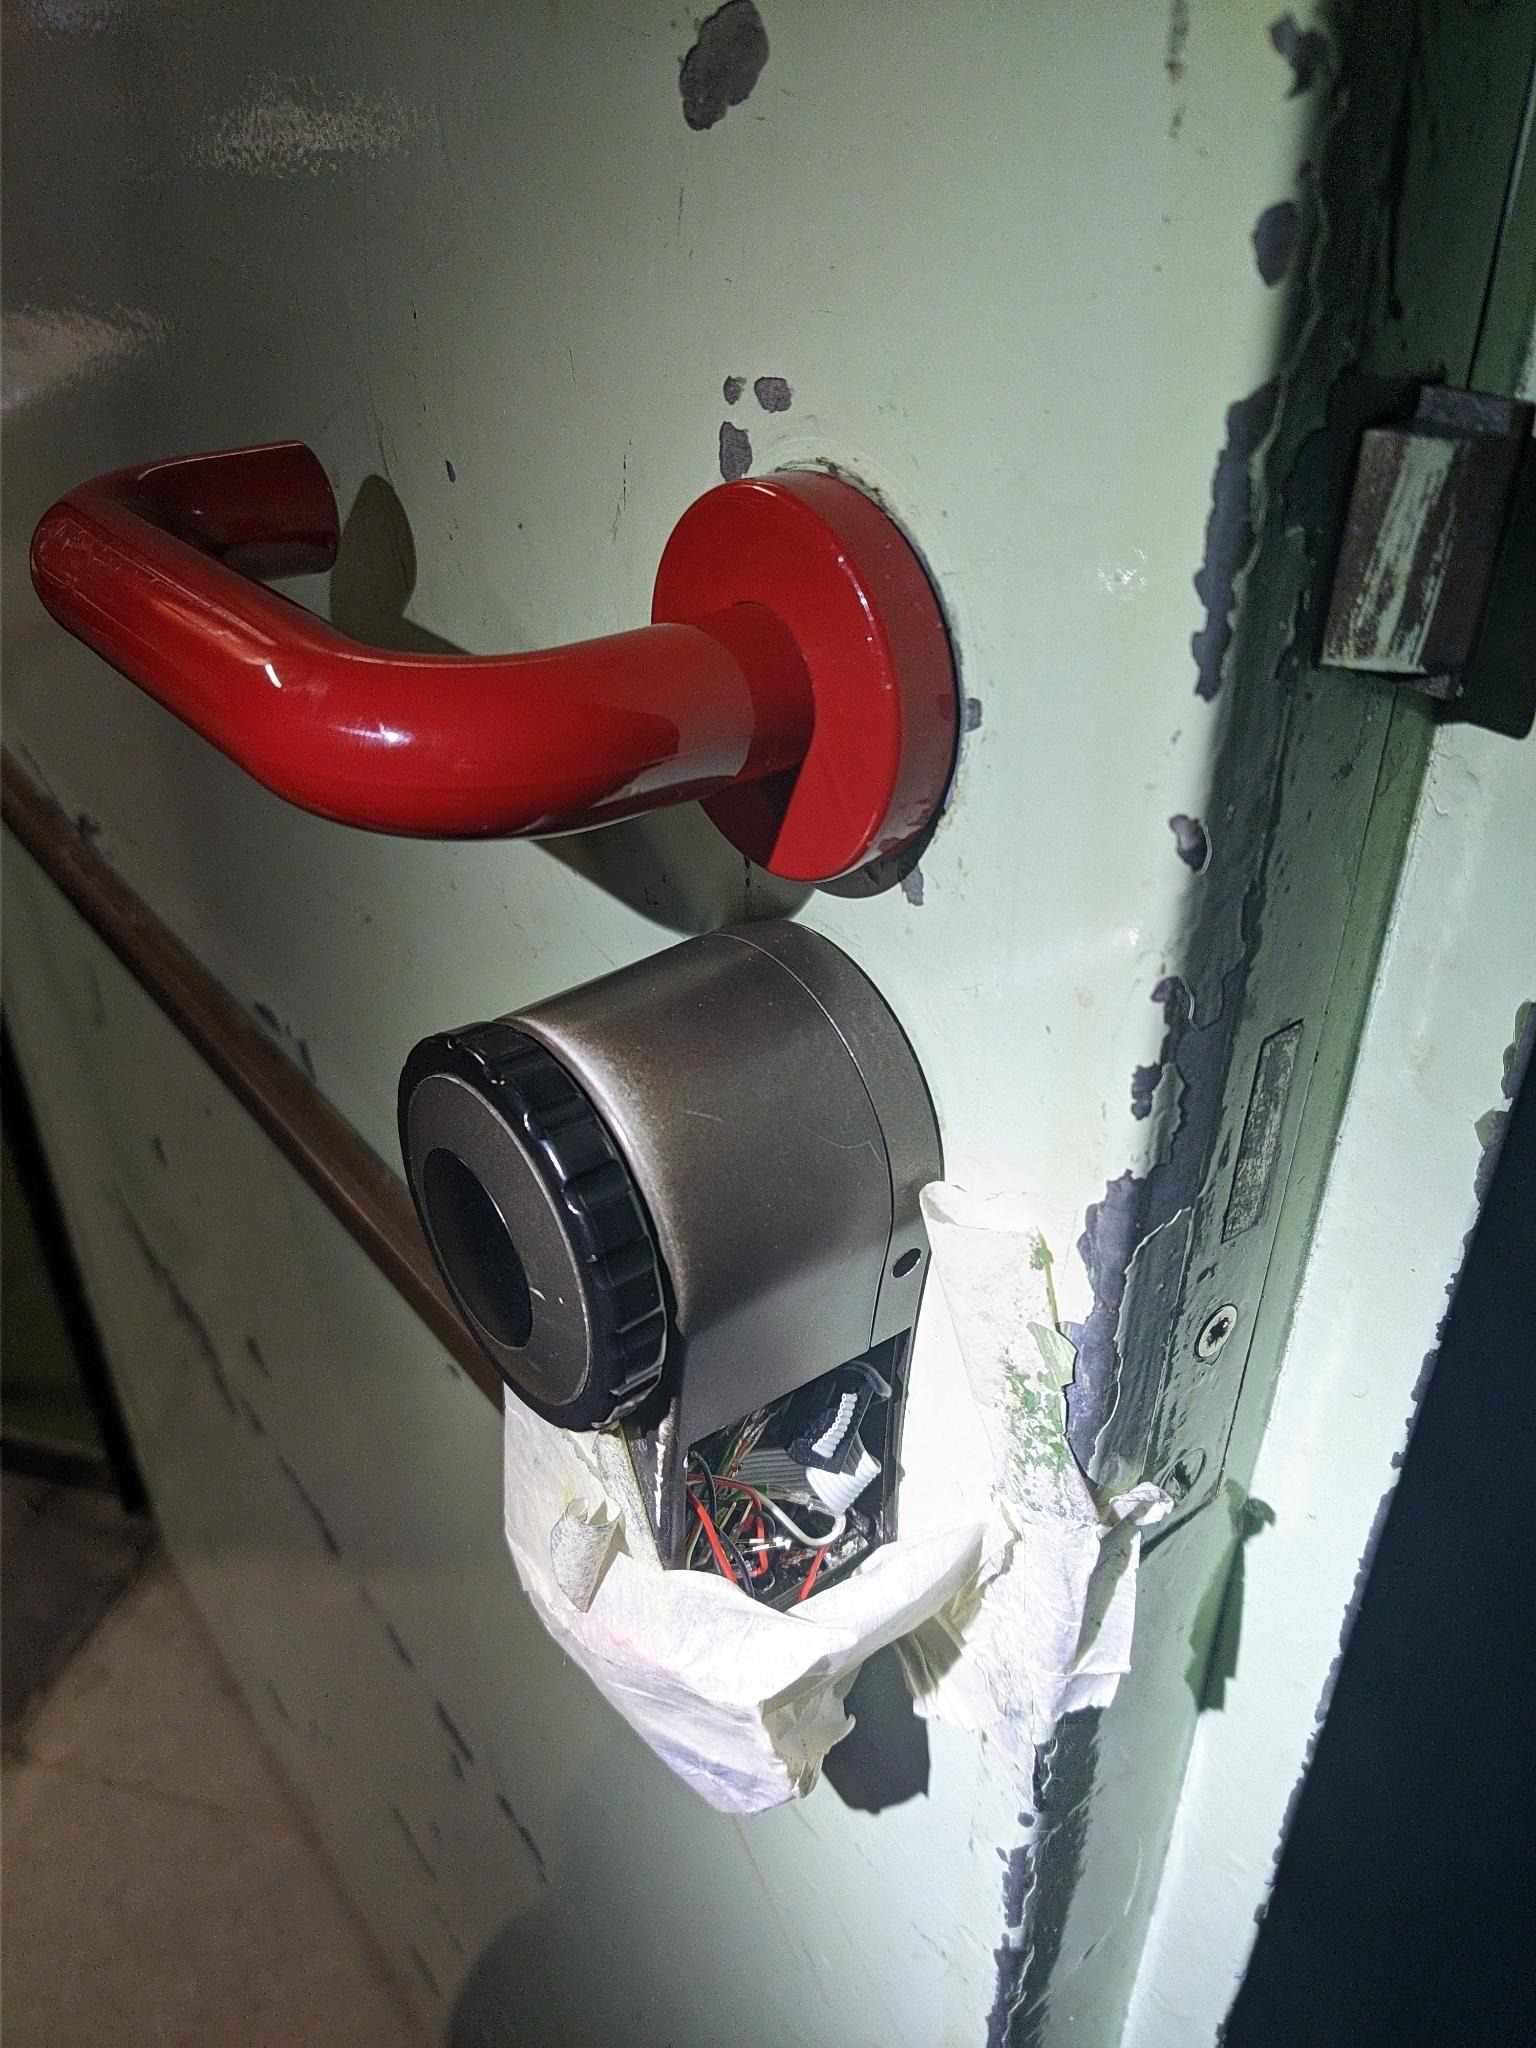
\includegraphics[height=0.75\textheight]{CFA1000-door.jpg}
\end{frame}

\begin{frame}
	\frametitle{... then a CNC mill arrived}

	\begin{center}
		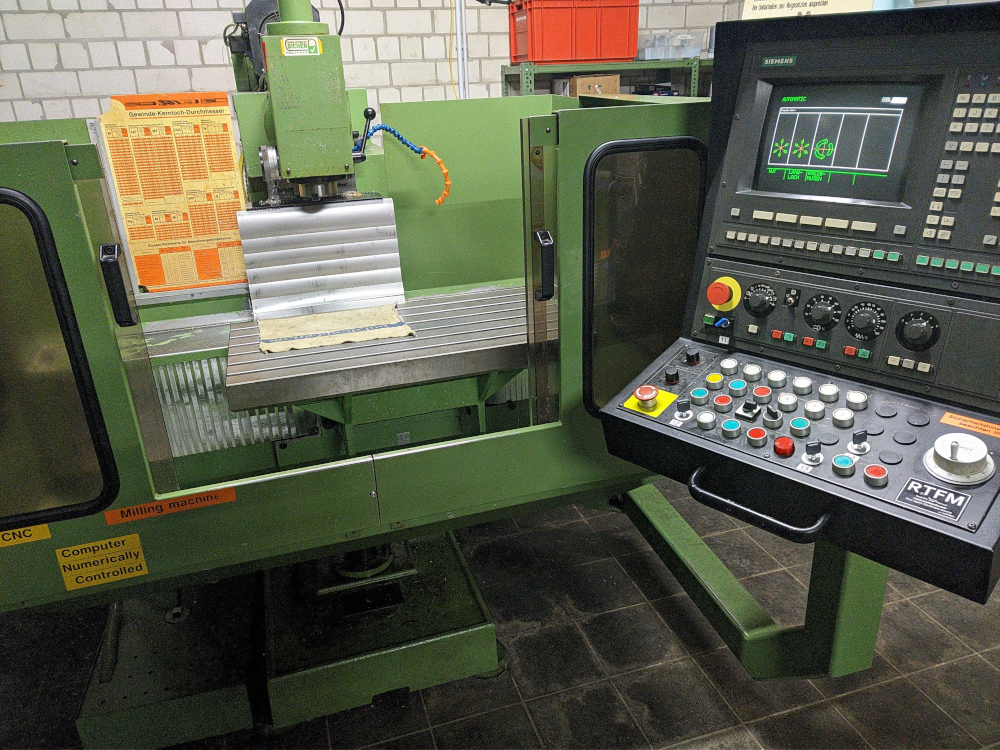
\includegraphics[height=0.8\textheight]{cnc-mill.jpg}
	\end{center}

\end{frame}

\begin{frame}
	\frametitle{CFA3000 - Using AES?}

	\begin{center}
		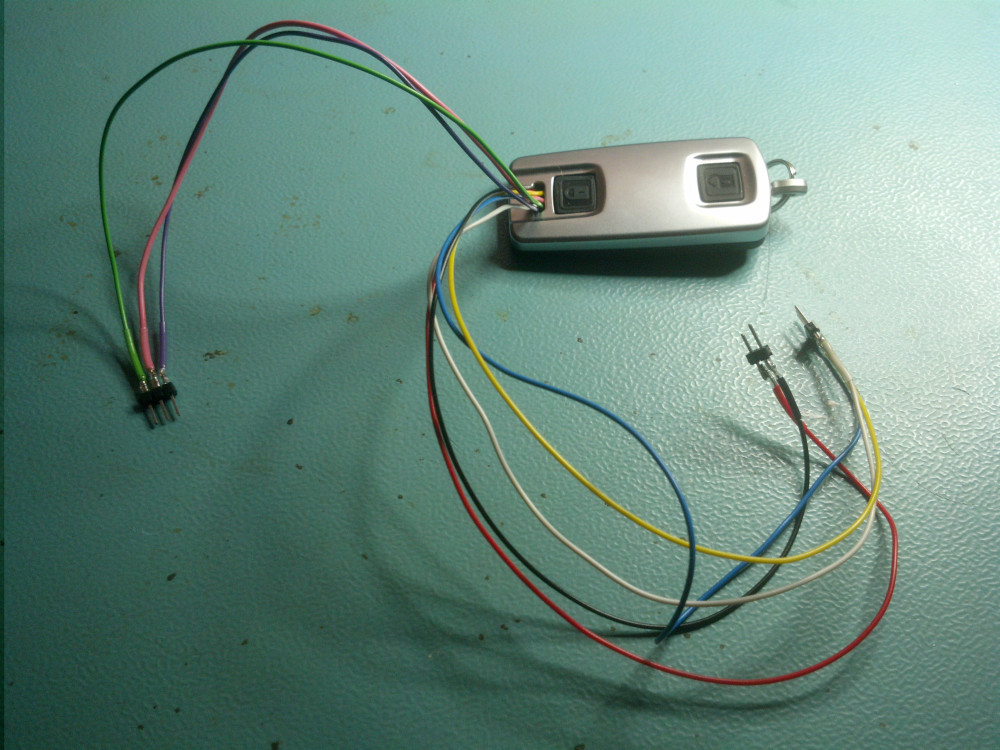
\includegraphics[height=0.55\textheight]{cfa3000-remote-control.jpg}
		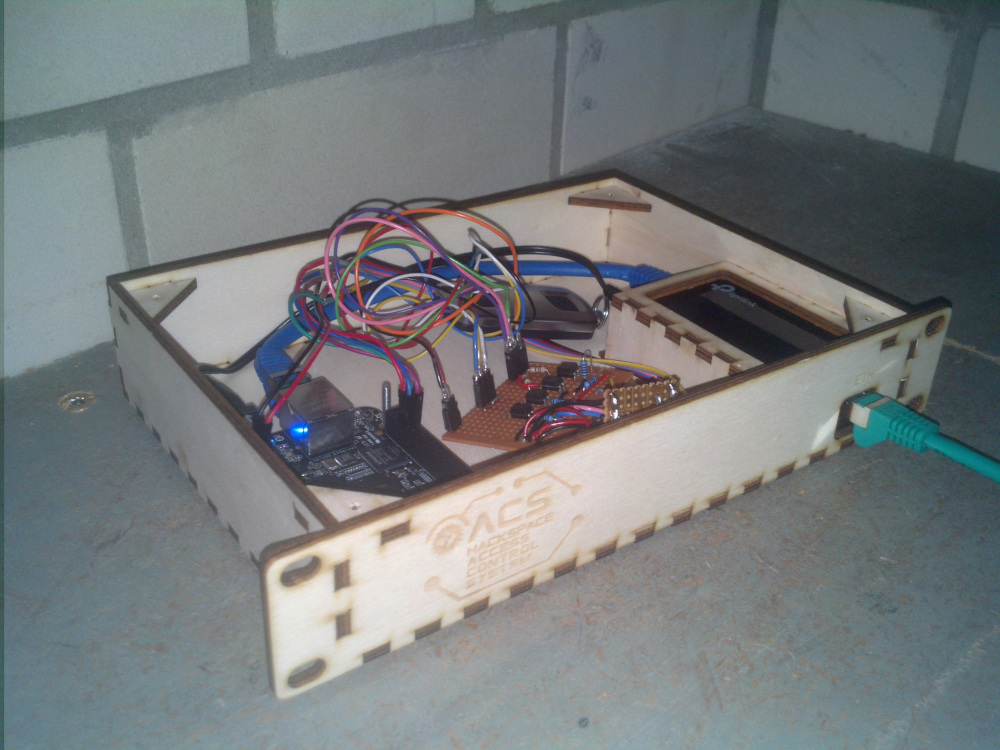
\includegraphics[height=0.55\textheight]{cfa3000-rev1.jpg}
	\end{center}
\end{frame}

\section{RF Analysis}

\begin{frame}
	\frametitle{SDR - Waterfall Plot}

	\begin{columns}
		\begin{column}{0.42\textwidth}
			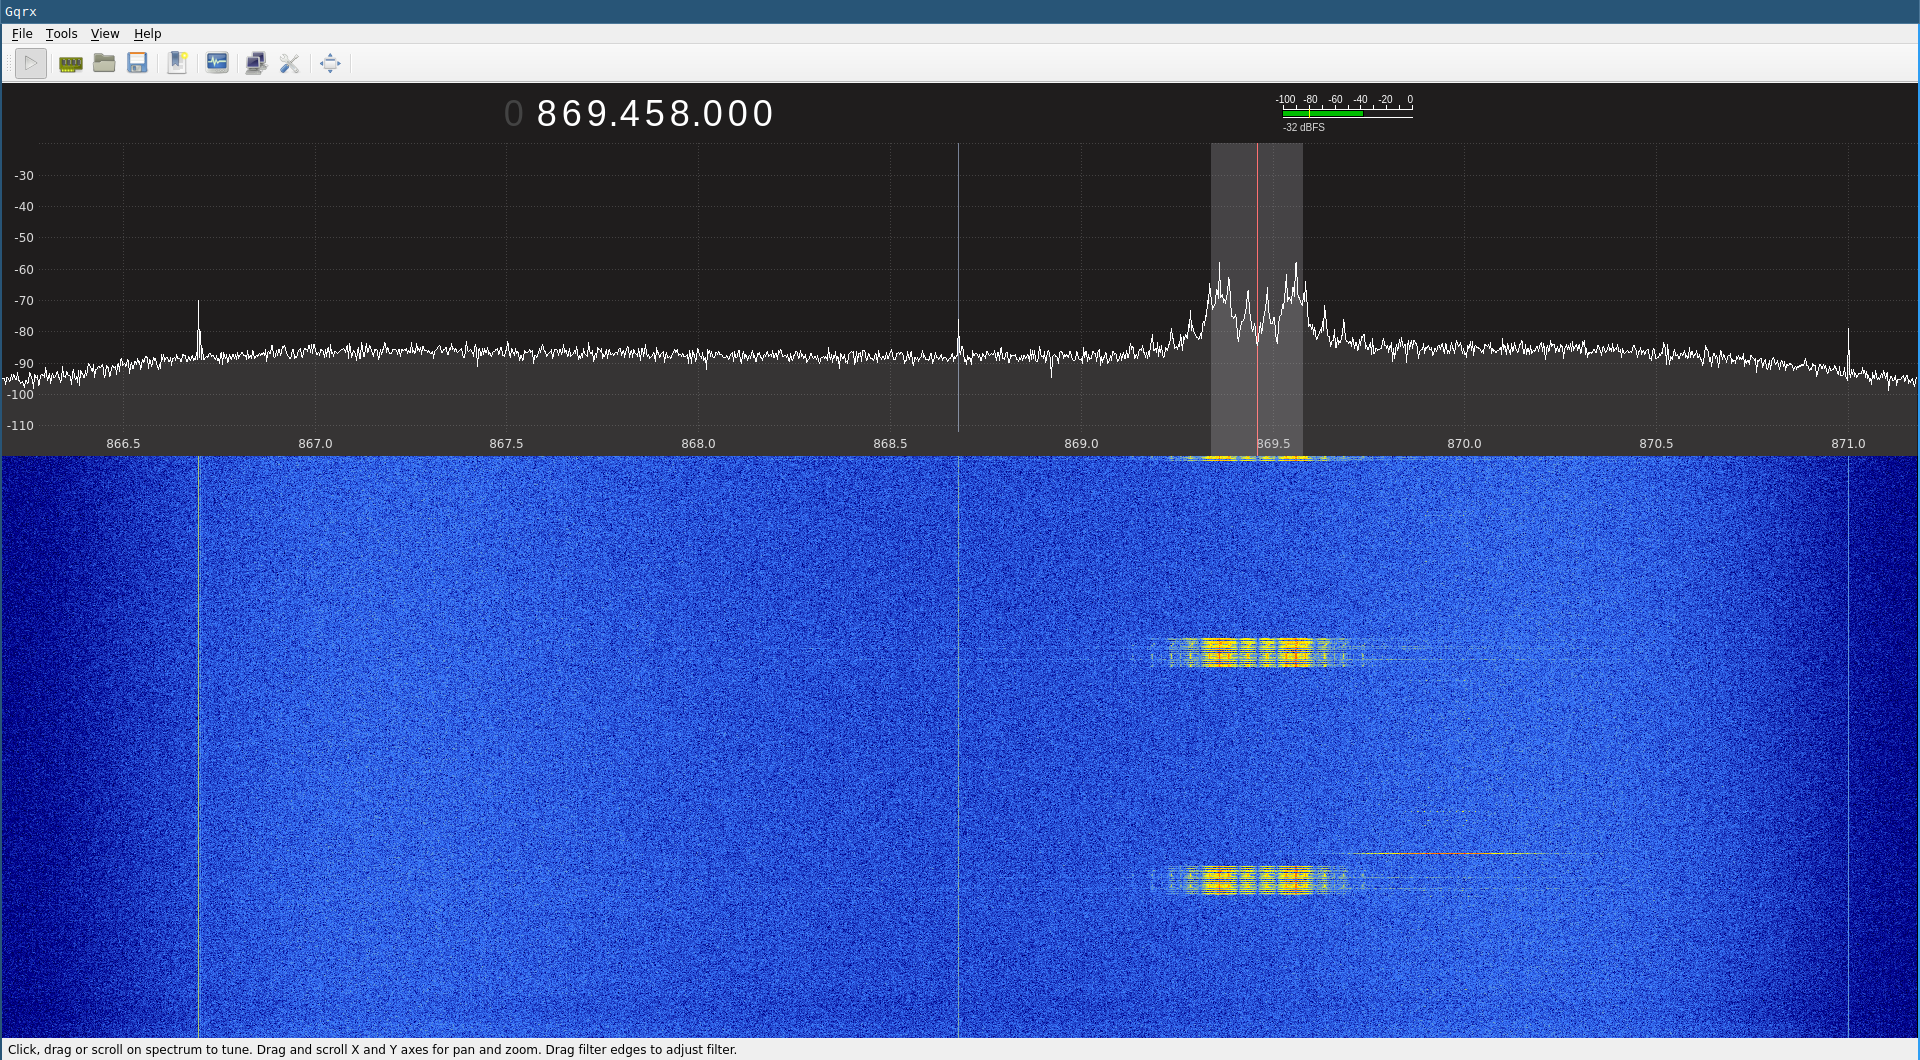
\includegraphics[width=1.0\textwidth]{gqrx-waterfall.png}
		\end{column}
		\begin{column}{0.58\textwidth}
			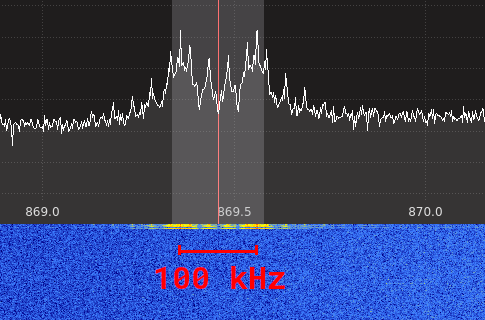
\includegraphics[width=1.0\textwidth]{gqrx-waterfall-fsk-100khz.png}
		\end{column}
	\end{columns}
\end{frame}

\begin{frame}
	\frametitle{FSK Demodulation}

	\begin{center}
		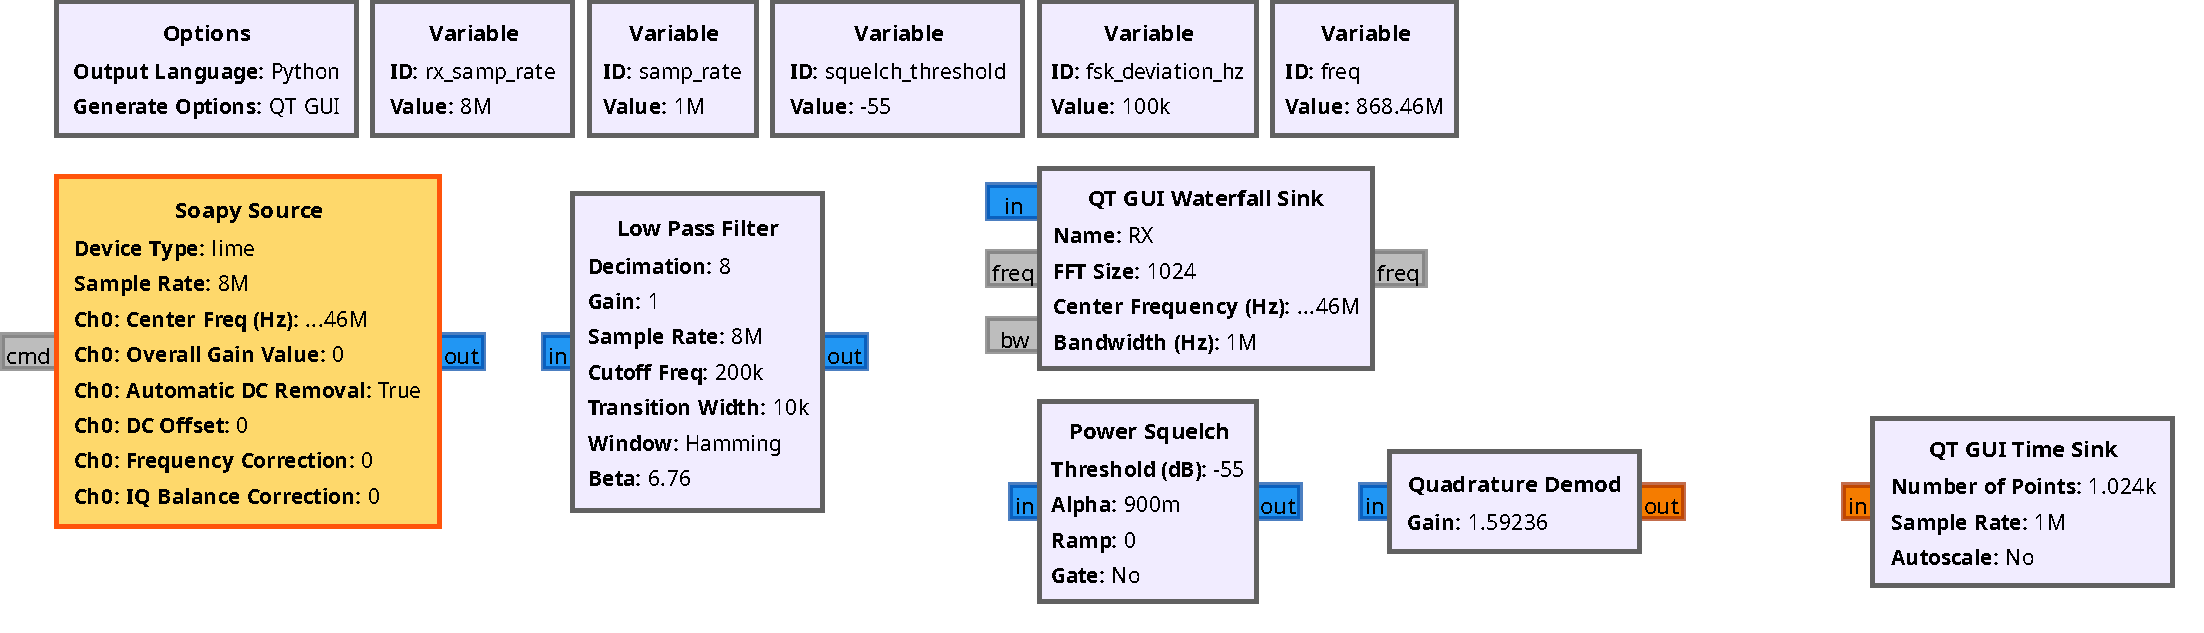
\includegraphics[width=0.95\textwidth]{gnuradio-fsk-demodulation.pdf}
	\end{center}
\end{frame}

\begin{frame}
	\frametitle{FSK Demodulation}

	\begin{center}
		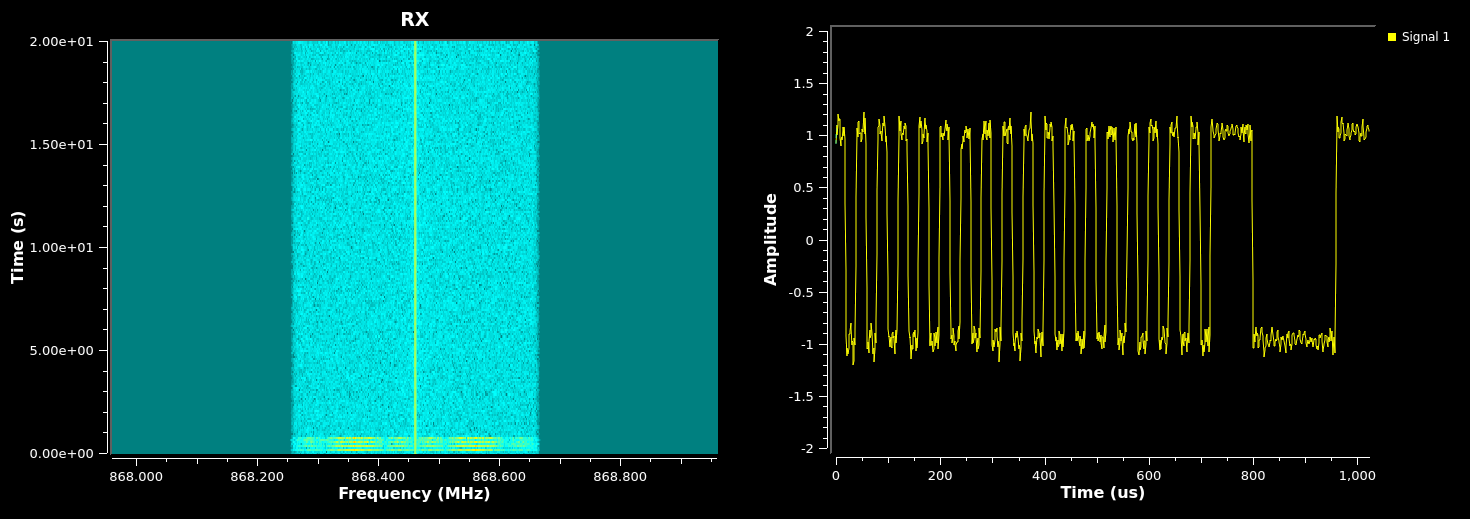
\includegraphics[width=1.0\textwidth]{gnuradio-post-demodulation.png}
	\end{center}
\end{frame}

\begin{frame}
	\frametitle{Baudrate Recovery}

	\begin{center}
		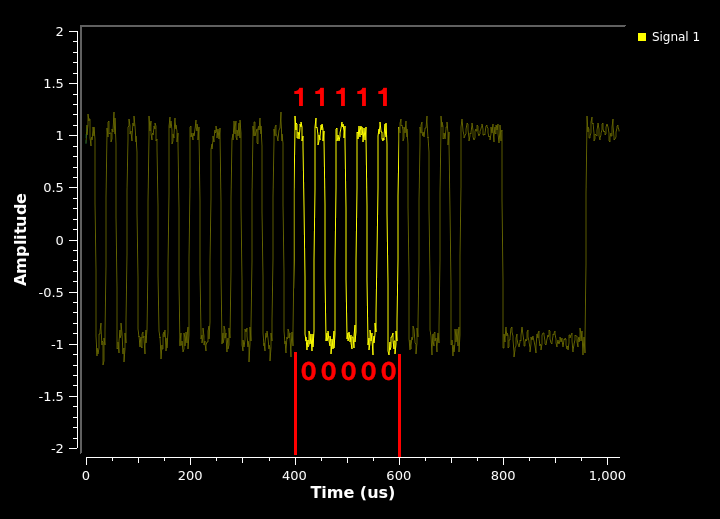
\includegraphics[height=0.8\textheight]{gnuradio-post-demodulation-timings.png}
	\end{center}

	\begin{itemize}
		\item In 200us there are 10 bits $\Rightarrow$ baudrate is 50k
	\end{itemize}
\end{frame}

\begin{frame}
	\frametitle{Symbol Synchronization}

	\begin{center}
		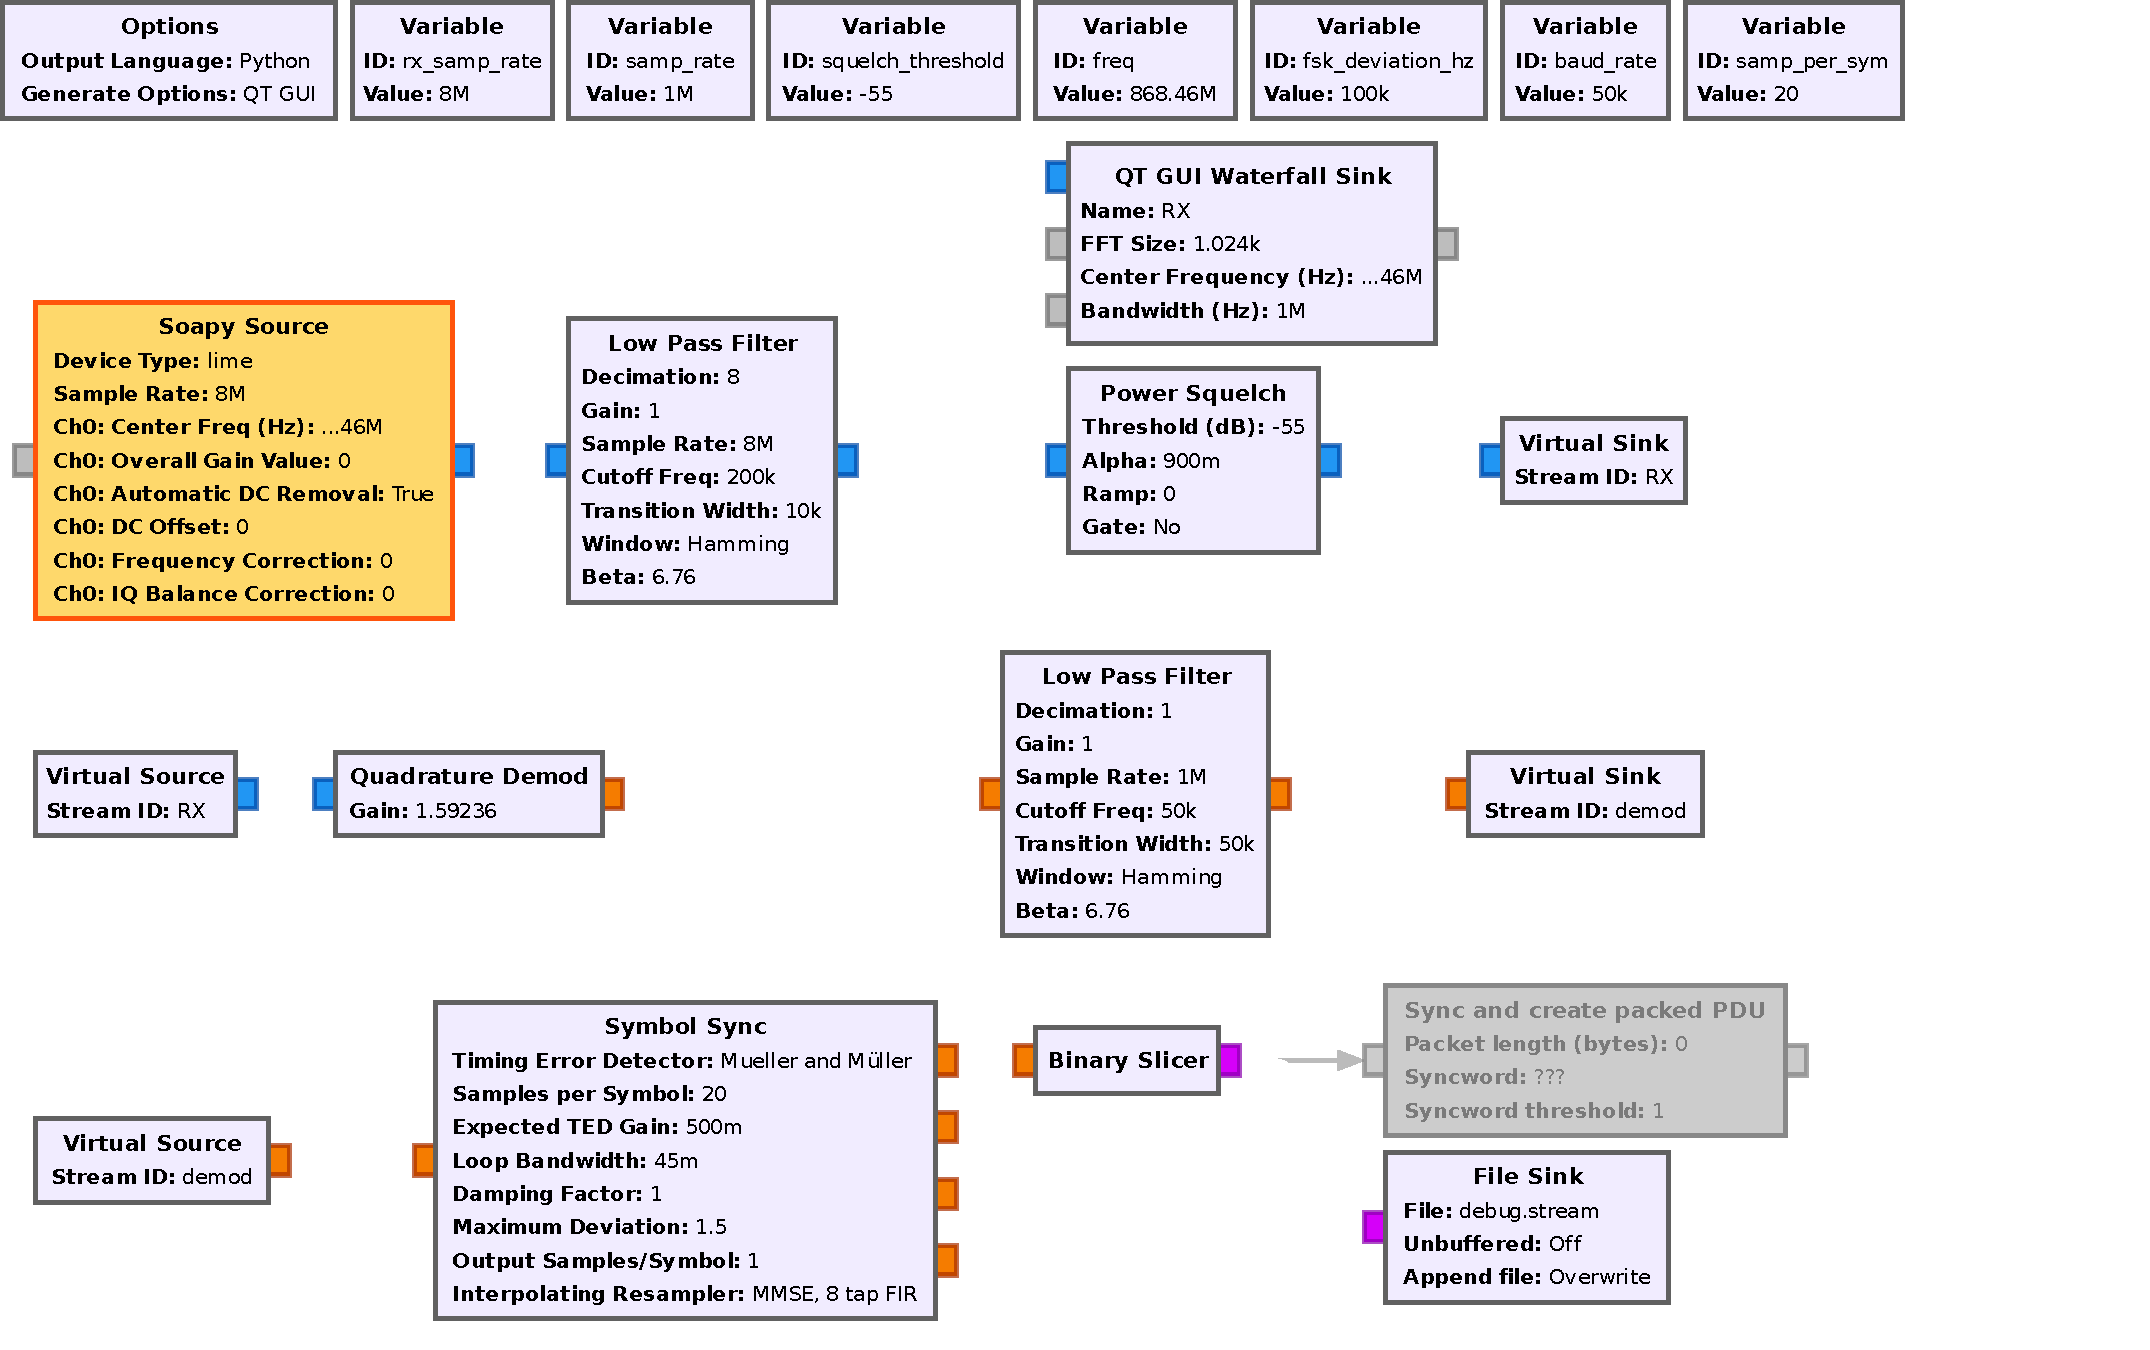
\includegraphics[height=0.9\textheight]{gnuradio-symbol-synchronized-dark.pdf}
	\end{center}
\end{frame}

\begin{frame}
	\frametitle{Message Header Recovery}

	\begin{itemize}
		\item Identified Packet Synchronization Header:
			\begin{itemize}
				\item \textbf{AA AA F0 0F 12 ED}
			\end{itemize}
		\item Identified Packet Length:
			\begin{itemize}
				\item \textbf{24 (total) - 6 (sync. header) = 18 [byte]}
			\end{itemize}
	\end{itemize}
\end{frame}

\begin{frame}
	\frametitle{Complete SDR Receiver}

	\begin{center}
		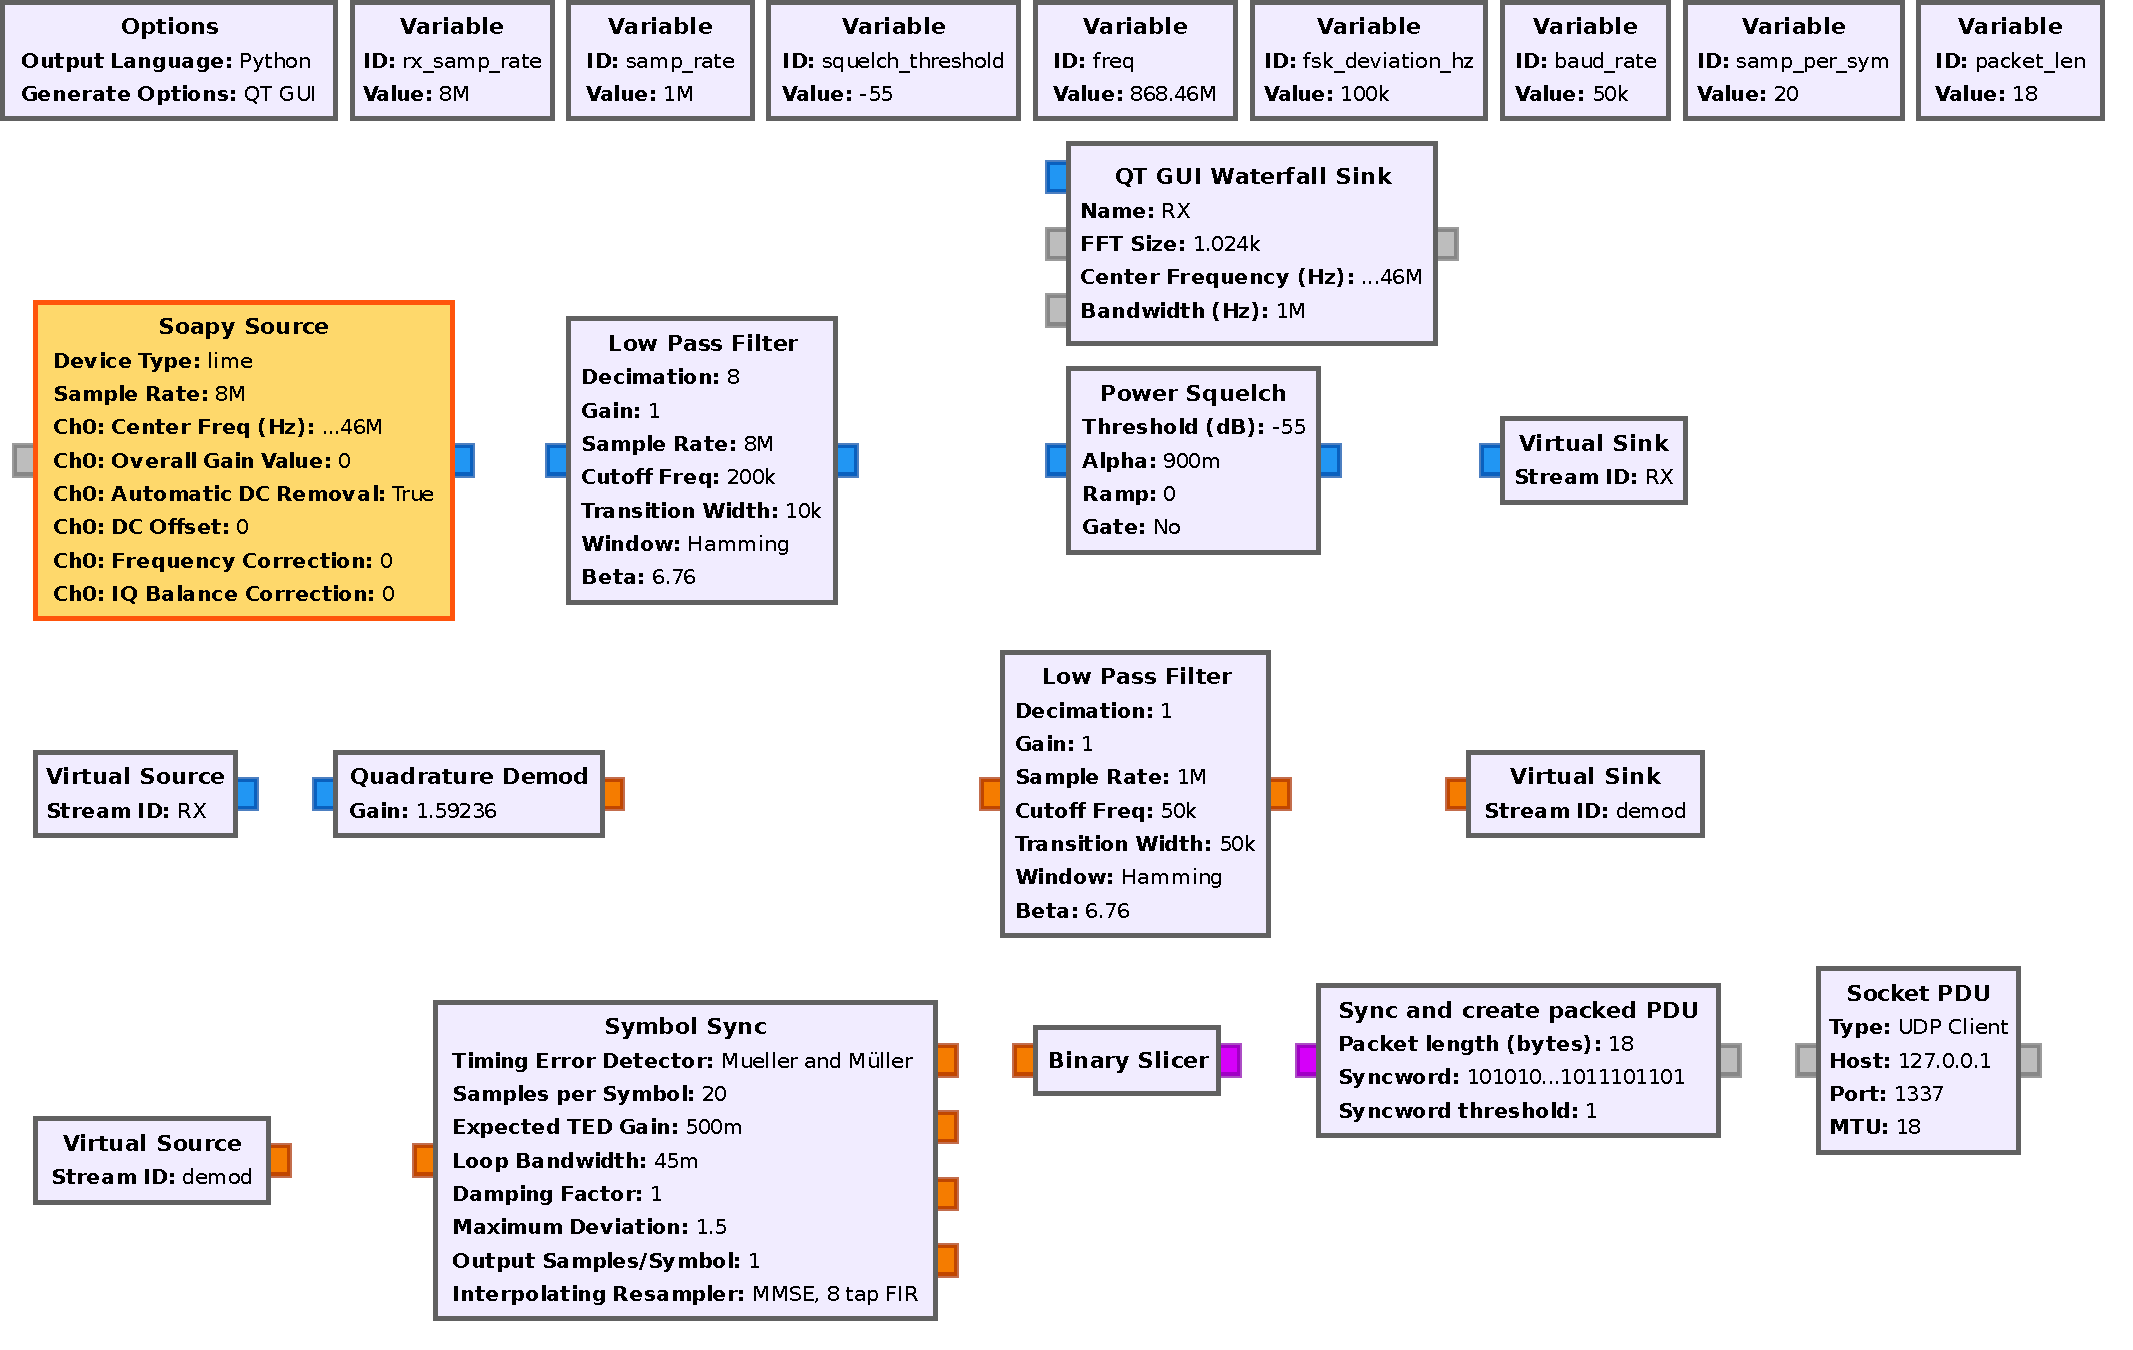
\includegraphics[height=0.9\textheight]{gnuradio-receiver-dark.pdf}
	\end{center}
\end{frame}

\section{Protocol analysis}
\begin{frame}[fragile]
	\frametitle{Packet Analysis}

	\begin{itemize}
		\item Next step: Making sense of the received packets
		\item The following python code dumps messages received by the previously described SDR toolchain
	\end{itemize}

\begin{scriptsize}
\begin{lstlisting}[frame=single,showstringspaces=false,language=Python,commentstyle=\color{commentsColor}\textit,keywordstyle=\color{keywordsColor}\bfseries,stringstyle=\color{stringColor}]
#!/usr/bin/python3
import socket

def printmsg(msg):
    print(' '.join(["{:02x}".format(x) for x in msg]))

sock = socket.socket(socket.AF_INET, socket.SOCK_DGRAM)
sock.bind(("127.0.0.1", 1337))

while True:
    printmsg(sock.recv(18))
\end{lstlisting}
\end{scriptsize}
\end{frame}

\begin{frame}
	\frametitle{Packet Analysis: Raw Data (from remote control)}

\begin{scriptsize}
\begin{tabular}{cccccccc>{\columncolor[RGB]{42, 42, 42}}cccccccc>{\columncolor[RGB]{42, 42, 42}}c>{\columncolor[RGB]{42, 42, 42}}c}
0 & 1 & 2 & 3 & 4 & 5 & 6 & 7 & 8 & 9 & a & b & c & d & e & f & 10 & 11\\
\hline
54 & 3d & 15 & 99 & 69 & 7b & 29 & 05 & 34 & 5e & 4b & 9c & 0e & e9 & ea & 50 & 2c & 20\\
54 & 3d & 15 & 99 & 69 & 7b & 29 & 05 & 35 & 5e & 4b & 9c & 0e & e9 & ea & 50 & 6b & f3\\
54 & 3d & 15 & 99 & 69 & 7b & 29 & 05 & 36 & 5e & 4b & 9c & 0e & e9 & ea & 50 & a3 & 86\\
54 & 3d & 15 & 99 & 69 & 7b & 29 & 05 & 37 & 5e & 4b & 9c & 0e & e9 & ea & 50 & e4 & 55\\
54 & 3d & 15 & 99 & 69 & 7b & 29 & 05 & 08 & 5e & 4b & 9c & 0e & e9 & ea & 50 & 7b & 4b\\
54 & 3d & 15 & 99 & 69 & 7b & 29 & 05 & 09 & 5e & 4b & 9c & 0e & e9 & ea & 50 & 3c & 98\\
54 & 3d & 15 & 99 & 69 & 7b & 29 & 05 & 0a & 5e & 4b & 9c & 0e & e9 & ea & 50 & f4 & ed\\
54 & 3d & 15 & 99 & 69 & 7b & 29 & 05 & 0b & 5e & 4b & 9c & 0e & e9 & ea & 50 & b3 & 3e\\
54 & 3d & 15 & 99 & 69 & 7b & 29 & 05 & 0c & 5e & 4b & 9c & 0e & e9 & ea & 50 & 74 & 26\\
...\\
\end{tabular}
\end{scriptsize}

	\begin{itemize}
		\item Data scrambled?
		\item Ends with CRC?
	\end{itemize}
\end{frame}

\begin{frame}
	\frametitle{CFF3000 Hardware}
		\begin{center}
			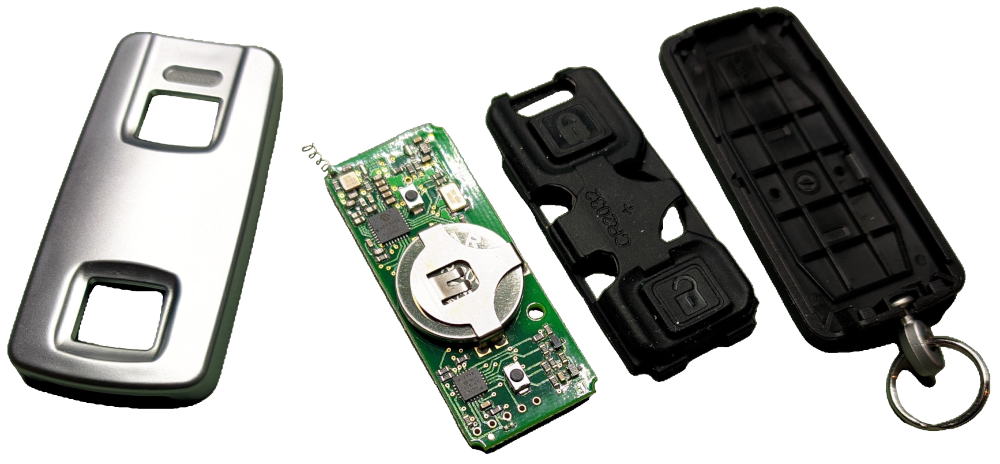
\includegraphics[width=0.6\textwidth]{cff3000-opened.png}
			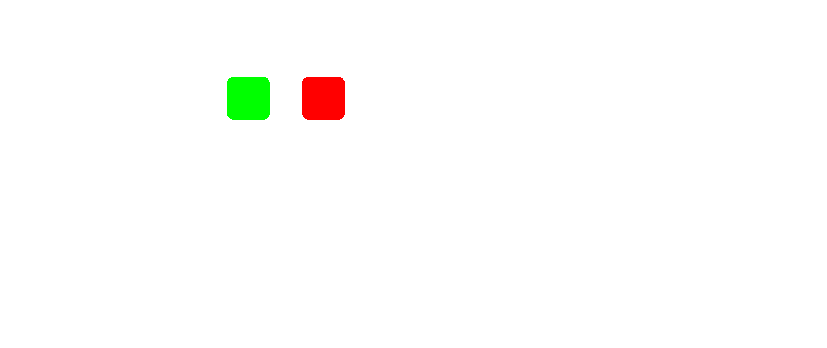
\includegraphics[width=0.6\textwidth]{cff3000-block-diagram.pdf}
		\end{center}
\end{frame}

\begin{frame}
	\frametitle{MRF89XA}

	\begin{columns}
		\begin{column}{0.3\textwidth}
			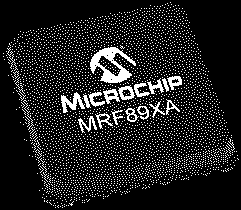
\includegraphics[width=1.0\textwidth]{mrf89xa-dithered.png}
		\end{column}
		\begin{column}{0.7\textwidth}
			\begin{itemize}
				\item MRF89XA has HW support
					\begin{itemize}
						\item Automatic CRC generation
						\item Two optional encodings
						\begin{itemize}
							\item Manchester encoding
							\item Linear feedback shift register polynomial $x^9 + x^5 + 1$
						\end{itemize}
					\end{itemize}
				\item In manchester encoding there can't be more than 2 sequential identical bits
					\begin{itemize}
						\item Received packets contained e.g. 0x3d or 0x7b, which has 4 sequential '1' bits
						\item $\Rightarrow$ \textbf{No manchster encoding}
					\end{itemize}
			\end{itemize}
		\end{column}
	\end{columns}

\end{frame}

\begin{frame}[fragile]
	\frametitle{Dewhite + CRC}

\begin{scriptsize}
\begin{tabular}{cccccccc>{\columncolor[RGB]{42, 42, 42}}ccccccccc}
0 & 1 & 2 & 3 & 4 & 5 & 6 & 7 & 8 & 9 & a & b & c & d & e & f & CRC\\
\hline
ab & ba & ad & c0 & de & da & e5 & 21 & 63 & 00 & 00 & 00 & 00 & 00 & 00 & 00 & OK\\
ab & ba & ad & c0 & de & da & e5 & 21 & 62 & 00 & 00 & 00 & 00 & 00 & 00 & 00 & OK\\
ab & ba & ad & c0 & de & da & e5 & 21 & 61 & 00 & 00 & 00 & 00 & 00 & 00 & 00 & OK\\
ab & ba & ad & c0 & de & da & e5 & 21 & 60 & 00 & 00 & 00 & 00 & 00 & 00 & 00 & OK\\
ab & ba & ad & c0 & de & da & e5 & 21 & 5f & 00 & 00 & 00 & 00 & 00 & 00 & 00 & OK\\
ab & ba & ad & c0 & de & da & e5 & 21 & 5e & 00 & 00 & 00 & 00 & 00 & 00 & 00 & OK\\
ab & ba & ad & c0 & de & da & e5 & 21 & 5d & 00 & 00 & 00 & 00 & 00 & 00 & 00 & OK\\
ab & ba & ad & c0 & de & da & e5 & 21 & 5c & 00 & 00 & 00 & 00 & 00 & 00 & 00 & OK\\
ab & ba & ad & c0 & de & da & e5 & 21 & 5b & 00 & 00 & 00 & 00 & 00 & 00 & 00 & OK\\
...\\
\end{tabular}
\end{scriptsize}

	\begin{itemize}
		\item 16 byte (128 bit) actual data
		\item Byte 8 contains a decrementing counter starting at 0x63 (99)
	\end{itemize}
\end{frame}

\begin{frame}
	\frametitle{Traffic between Remote Control and Door Lock}

	\begin{center}
		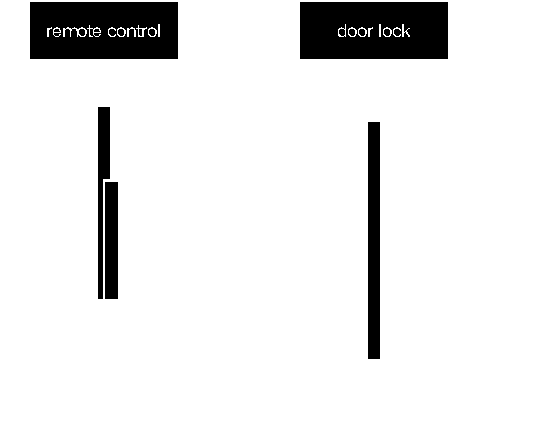
\includegraphics[width=0.6\textwidth]{communication.pdf}
	\end{center}
\end{frame}

\begin{frame}
	\frametitle{Message Format of Message A (initial key request)}

	\begin{center}
		\begin{tabular}{|c|c|c|c|c|c|}
			\hline
			\textbf{Byte}        & 0    & 1-6  & 7   & 8       & 9-15 \\
			\hline
			\textbf{Description} & 0xab & ADDR & CMD & Counter & 0x00 \\
			\hline
		\end{tabular}
	\end{center}

	\begin{itemize}
		\item 0xab = fixed byte, always 0xab
		\item ADDR = remote control specific address/ID
		\item CMD = command for the door (e.g. unlock or lock)
			\begin{itemize}
				\item \texttt{0x01} = Status Door
				\item \texttt{0x11} = Lock Door
				\item \texttt{0x21} = Unlock Door
			\end{itemize}
		\item Counter = Decrementing counter from 99 to 0
		\item 0x00 = fixed bytes, always 0x00
	\end{itemize}
\end{frame}

\begin{frame}
	\frametitle{Message Format of Message B (door response)}

	\begin{center}
		\begin{tabular}{|c|c|c|c|c|c|c|}
			\hline
			\textbf{Byte}        & 0    & 1-6  & 7   & 8-13 & 14 & 15 \\
			\hline
			\textbf{Description} & 0xab & ADDR & CMD & Challenge & Status & ??? \\
			\hline
		\end{tabular}
	\end{center}

	\begin{itemize}
		\item 0xab = fixed byte, always 0xab
		\item ADDR = inverted and nibble swapped remote control address
		\item CMD = command for the door (e.g. unlock or lock)
		\item Challenge = seems to be arbitrary data, changes on each request
		\item Status = Door Status (locked, unlocked)
			\begin{itemize}
				\item \texttt{0x00} = Door Status Unknown
				\item \texttt{0x02} = Door Status Unlocked
				\item \texttt{0x04} = Door Status Locked
			\end{itemize}
		\item ??? = not sure, might be Door Battery Status
	\end{itemize}
\end{frame}

\begin{frame}
	\frametitle{Message Format of Message C (final packet)}

	\begin{center}
		\begin{tabular}{|c|c|c|c|c|c|c|}
			\hline
			\textbf{Byte}        & 0-15 \\
			\hline
			\textbf{Description} & encrypted \\
			\hline
		\end{tabular}
	\end{center}

	\begin{itemize}
		\item Only send for (un)lock commands
		\item Sending same message B with fake CFA3000 generates same message C
	\end{itemize}
\end{frame}

\begin{frame}
	\frametitle{Traffic between Remote Control and Door Lock}

	\begin{center}
		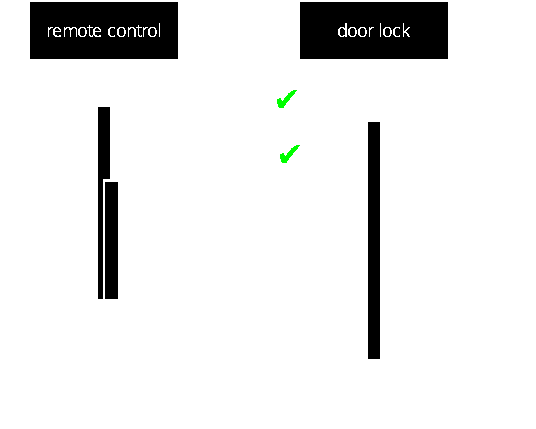
\includegraphics[width=0.6\textwidth]{communication2.pdf}
	\end{center}
\end{frame}

\begin{frame}
	\frametitle{Pairing}

	\begin{center}
		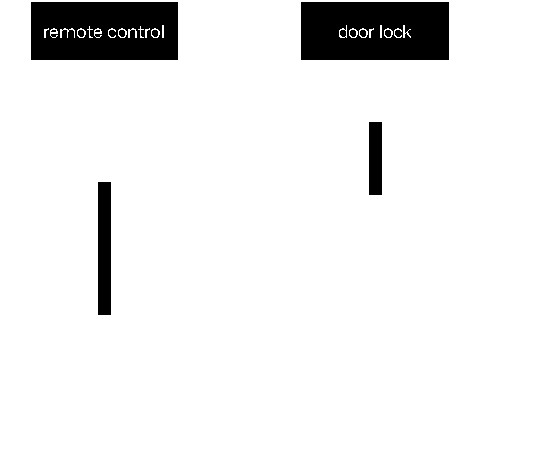
\includegraphics[width=0.6\textwidth]{pairing.pdf}
	\end{center}
\end{frame}

\begin{frame}
	\frametitle{I can haz c0de?}

	\begin{columns}
		\begin{column}{0.7\textwidth}
			\begin{itemize}
				\item PIC16LF1829
					\begin{itemize}
						\item Programming header easily available
						\item All protection bits are set
					\end{itemize}
				\item Only one memory block, so not affected by PIC locking fuse issue
				\item Power/Voltage glitching?
				\item Use Chinese service?
				\item Use scanning electron microscope to read bits?
			\end{itemize}
		\end{column}
		\begin{column}{0.3\textwidth}
			\begin{center}
				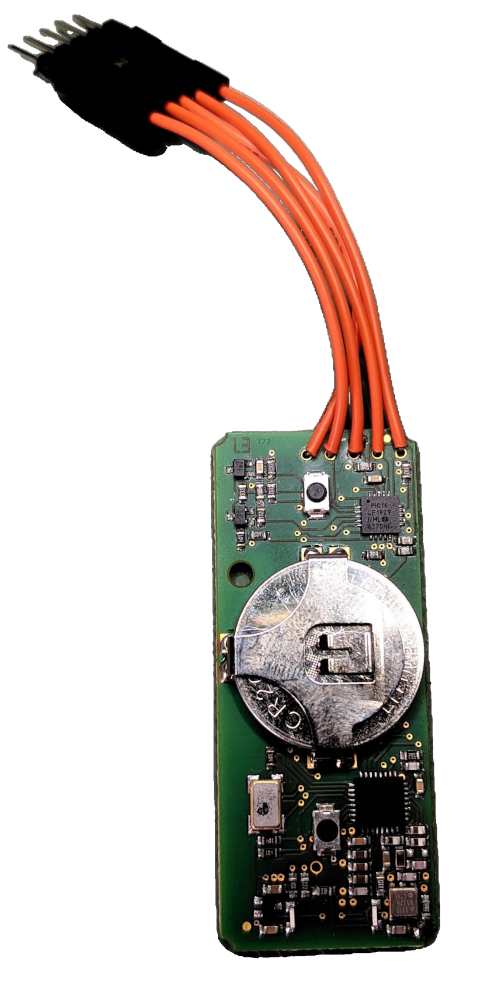
\includegraphics[width=0.8\textwidth]{cff3000-programmer.png}
			\end{center}
		\end{column}
	\end{columns}
\end{frame}

\begin{frame}
	\frametitle{We bought a broken Tesla BS300...}

	\begin{center}
		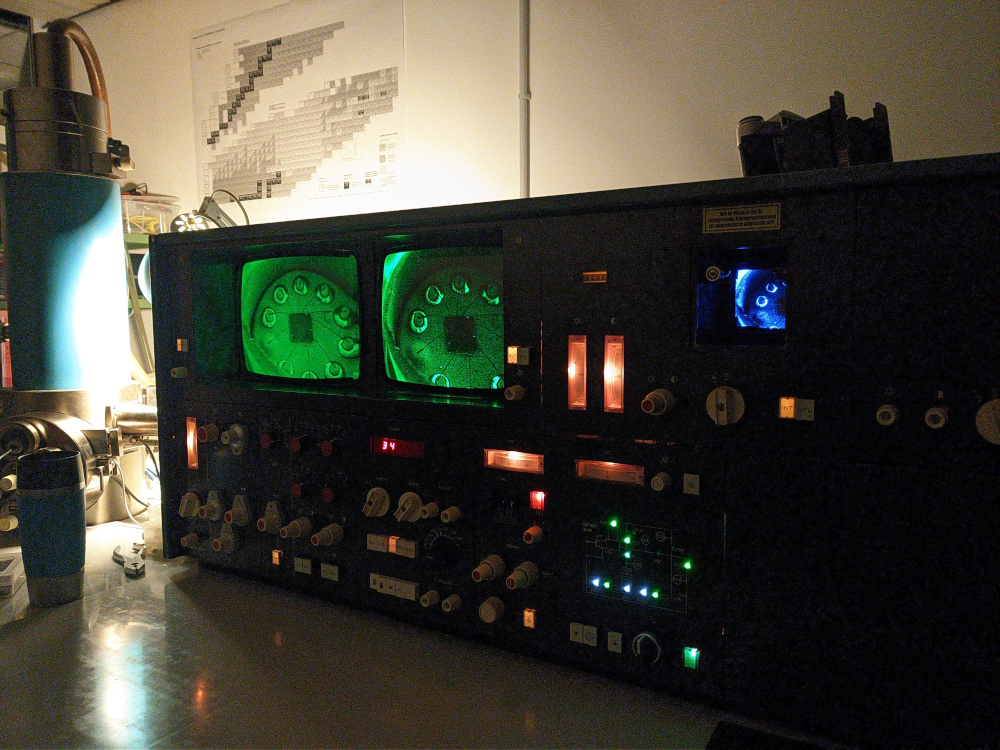
\includegraphics[height=0.9\textheight]{sem-01.jpg}
	\end{center}
\end{frame}

\begin{frame}
	\frametitle{... and got it running}

	\begin{center}
		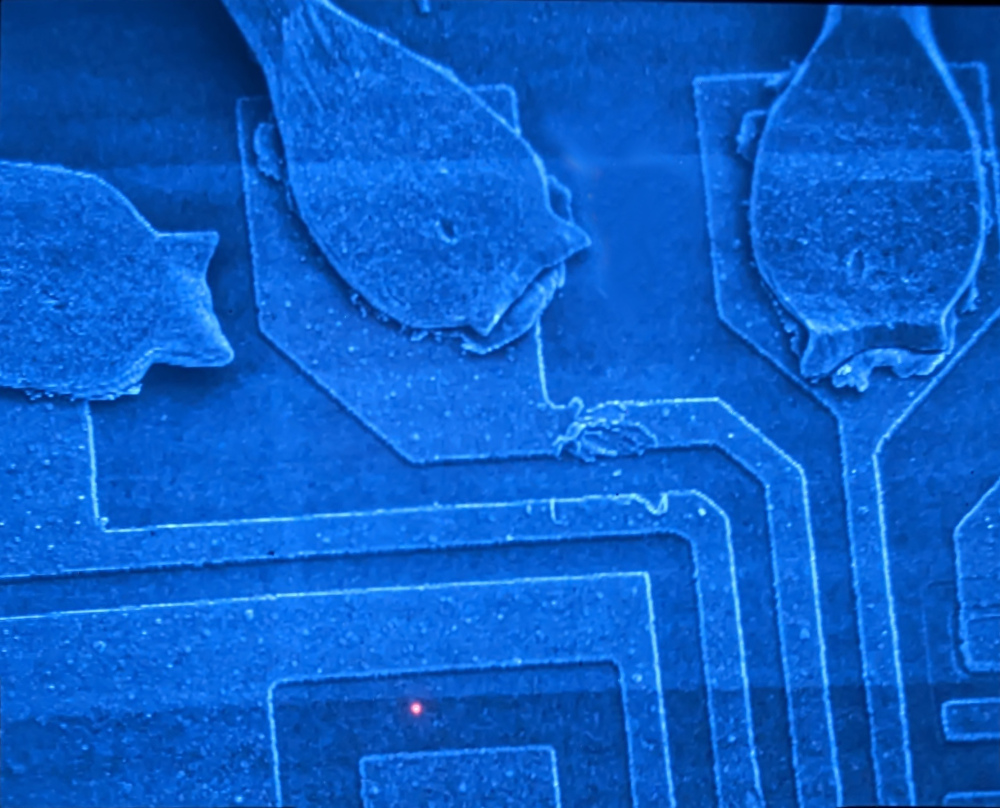
\includegraphics[height=0.6\textheight]{sem-02.jpg}
		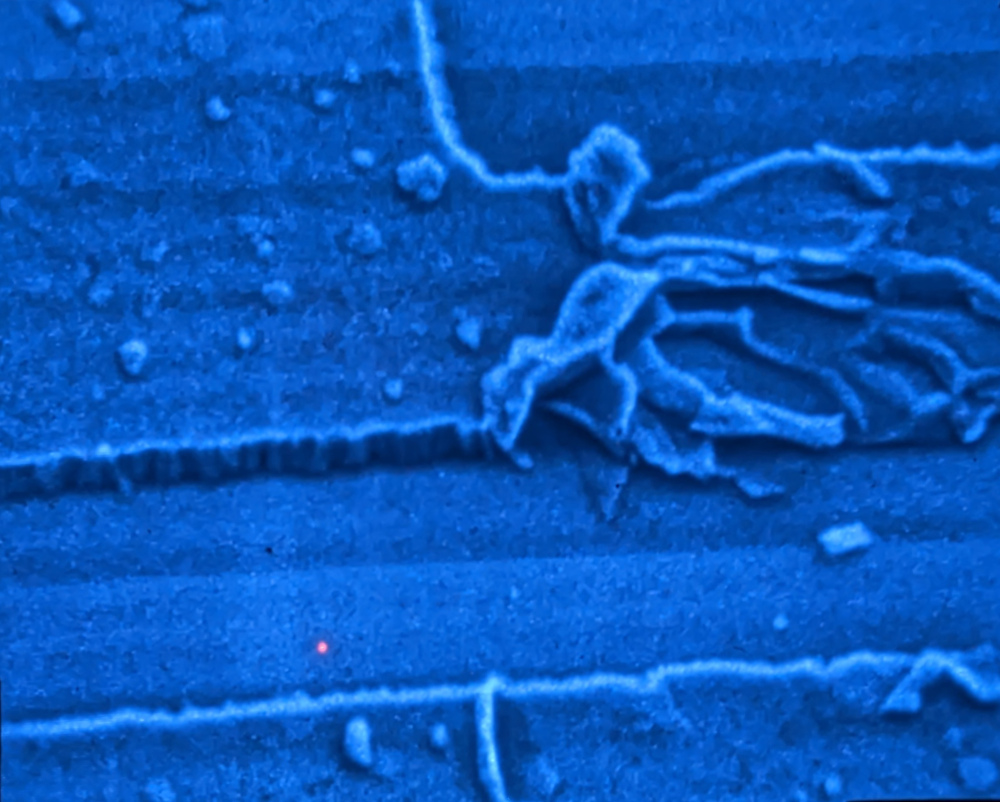
\includegraphics[height=0.6\textheight]{sem-03.jpg}
	\end{center}
\end{frame}

\begin{frame}
	\frametitle{But it needs lots of maintenance :(}

	\begin{center}
		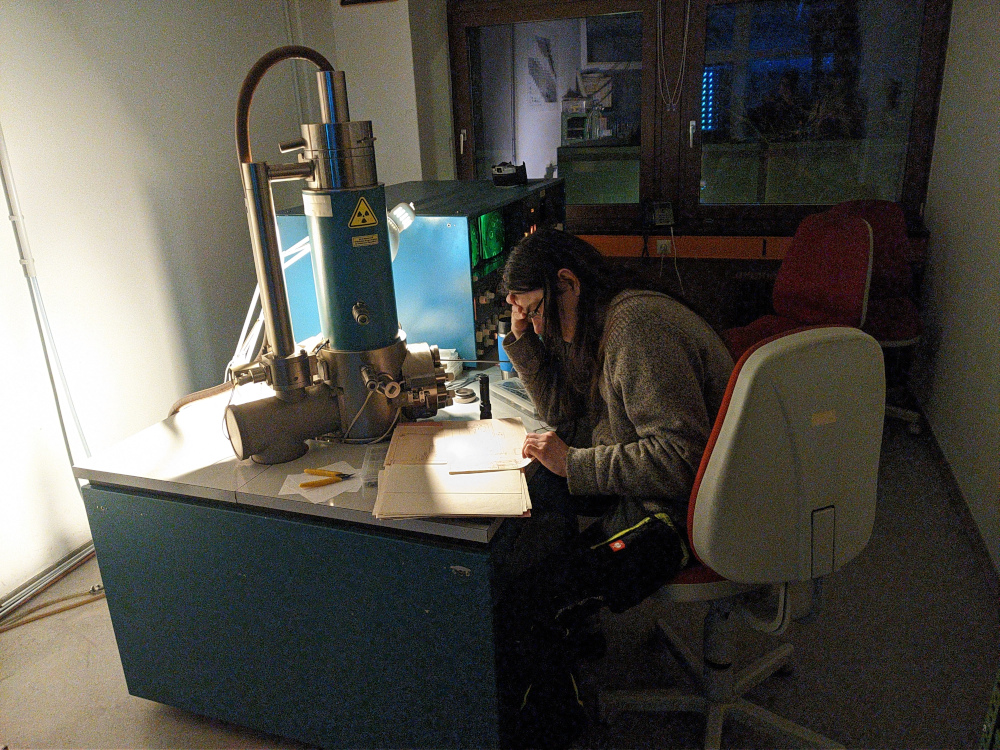
\includegraphics[height=0.9\textheight]{sem-04.jpg}
	\end{center}
\end{frame}

\begin{frame}
	\frametitle{Failed to decap chips :(}

	\begin{center}
		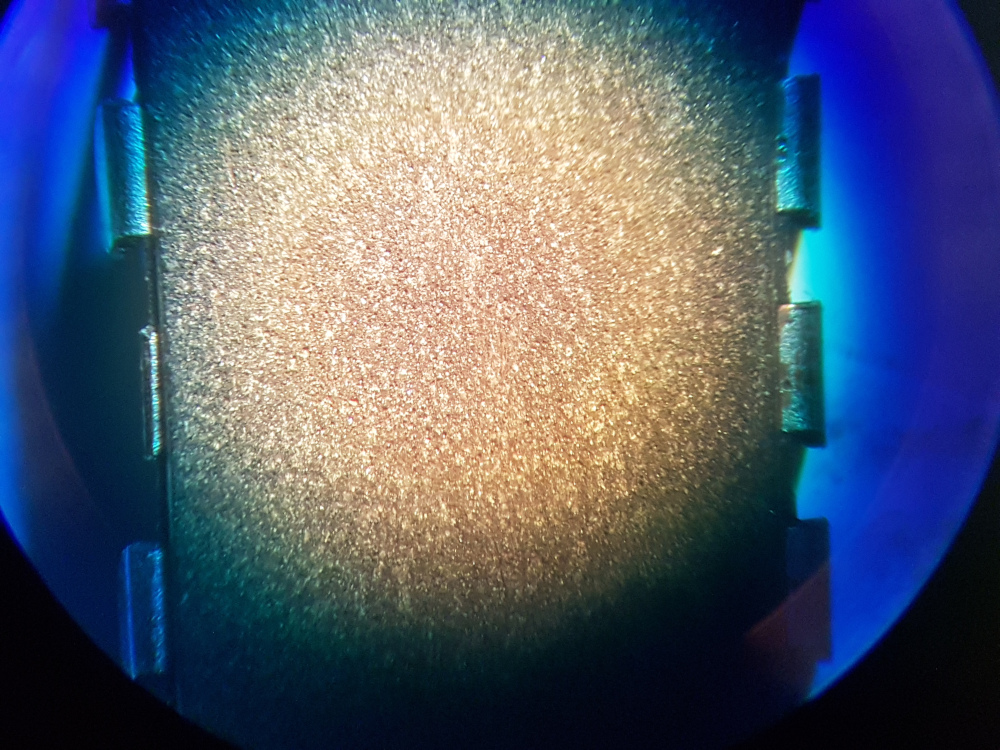
\includegraphics[height=0.9\textheight]{sem-05.jpg}
	\end{center}
\end{frame}

\begin{frame}
	\frametitle{CFA3000 has a PIC18LF45K80?!}

	\begin{center}
		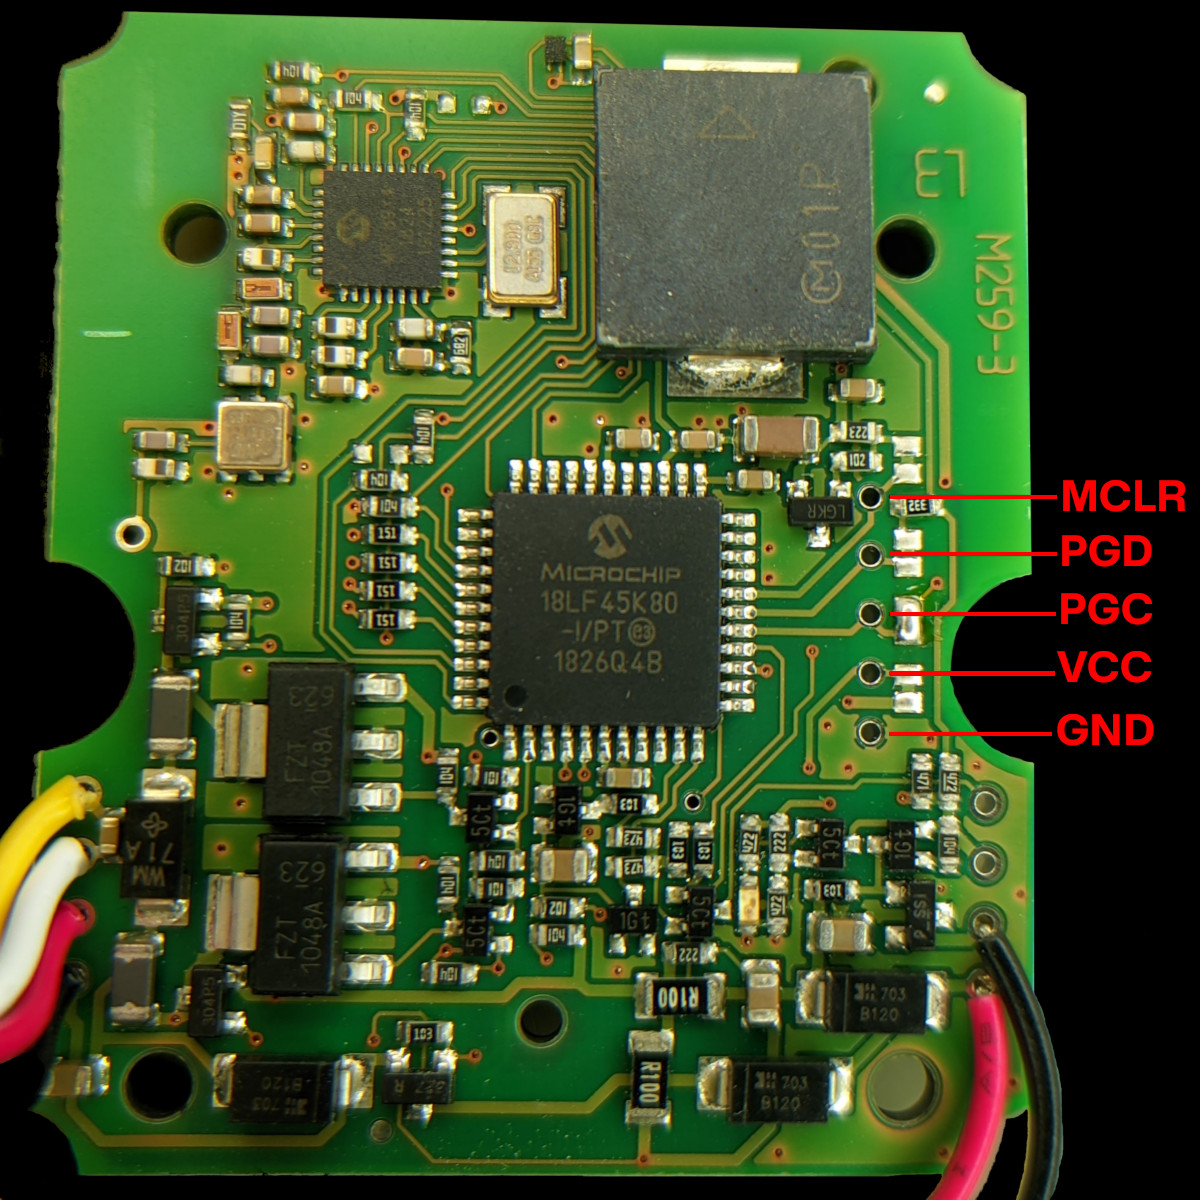
\includegraphics[height=0.9\textheight]{cfa3000-pcb.jpg}
	\end{center}
\end{frame}

\begin{frame}
	\frametitle{PIC18LF45K80 Breakout Board}

	\begin{center}
		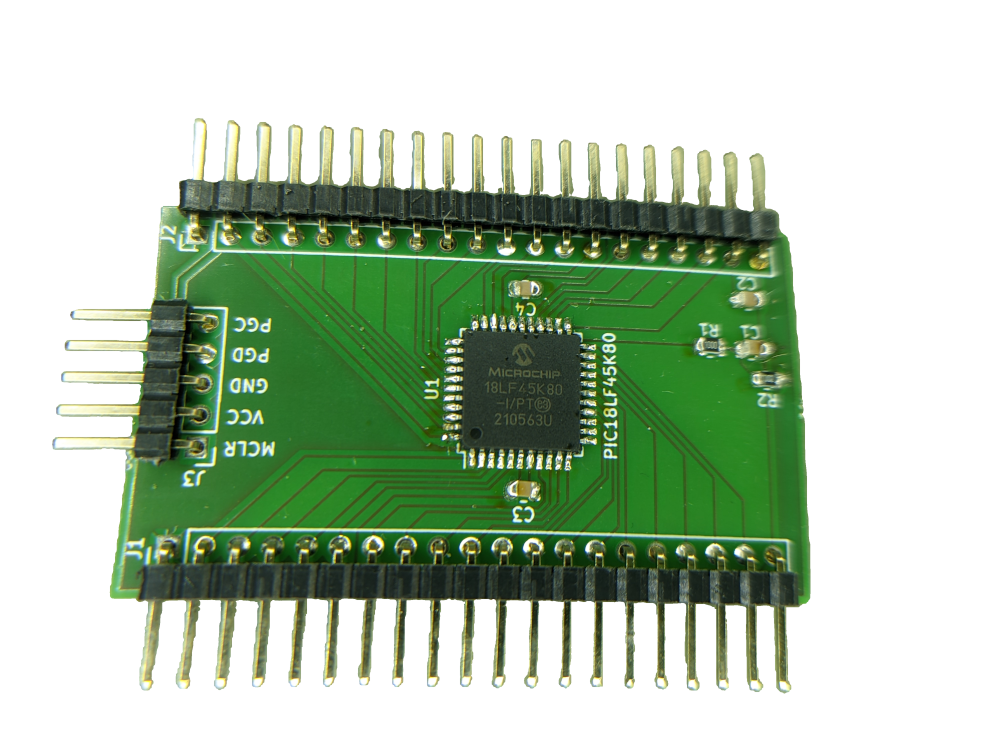
\includegraphics[width=0.7\textwidth]{pic-breakoutboard.png}
	\end{center}
\end{frame}

\begin{frame}
	\frametitle{Wire ICSP \& Serial}

	\begin{center}
		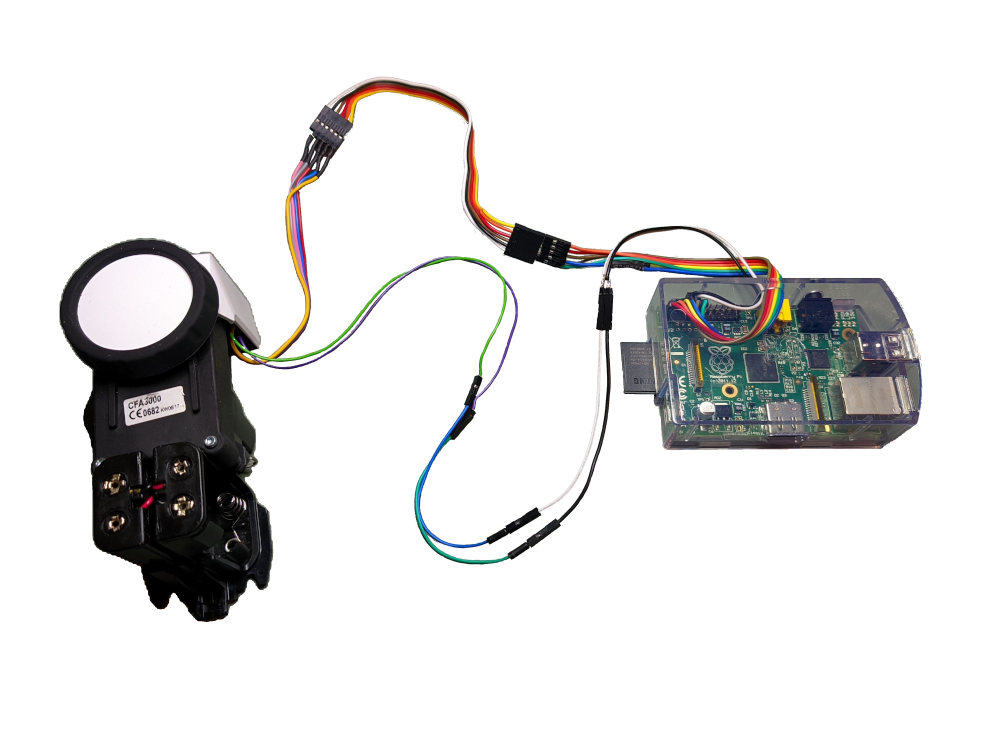
\includegraphics[height=1.0\textheight]{hardware-modification-02.png}
	\end{center}
\end{frame}

\begin{frame}
	\frametitle{PIC18LF45K80 Fuses}

	\begin{center}
		\begin{tabular}{|c|c|c|c|}
			\hline
			Block & Start & Stop & Protection Fuses \\
			\hline
			0 & 0x0000 & 0x1000 & CP, TBR, WP \\
			1 & 0x1000 & 0x2000 & \textbf{CP, WP} \\
			2 & 0x2000 & 0x4000 & CP, TBR, WP \\
			3 & 0x4000 & 0x6000 & CP, TBR, WP \\
			4 & 0x6000 & 0x8000 & CP, TBR, WP \\
			EEPROM & --- & --- & CP \\
			\hline
		\end{tabular}
	\end{center}

	\begin{itemize}
		\item CP = Code Protection (Blocks read via ICSP)
		\item WP = Write Protection
		\item TBR = Table Read Protection
	\end{itemize}

	\vspace{0.25cm}

	But \textbf{block 0 is not TBR protected} and can be dumped by overriding
	the first block using the same technique described in the Hörman Bisecur
	talk at 34C3.
\end{frame}

\begin{frame}[fragile]
	\frametitle{Dump Block 1}

	\begin{columns}
		\begin{column}{0.2\textwidth}
			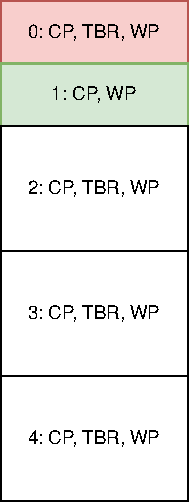
\includegraphics[width=1.0\textwidth]{block1.pdf}
		\end{column}
		\begin{column}{0.8\textwidth}
			\begin{enumerate}
				\item Erase block 0
				\item Write pseudo-code from below into block 0
				\item Get code/data dumped via serial
			\end{enumerate}

			\vspace{1cm}

\begin{scriptsize}
\begin{lstlisting}[frame=single,language=C,commentstyle=\color{commentsColor}\textit,keywordstyle=\color{keywordsColor}\bfseries,stringstyle=\color{stringColor}]
unsigned char buffer, *address;

serial_setup();
for (address=0x1000; address<0x2000; address++) {
    buffer = read_data(address);
    serial_putc(buffer);
}
\end{lstlisting}
\end{scriptsize}

		\end{column}
	\end{columns}

\end{frame}

\begin{frame}[fragile]
	\frametitle{TBLRD Fuse}

	\begin{columns}
		\begin{column}{0.2\textwidth}
			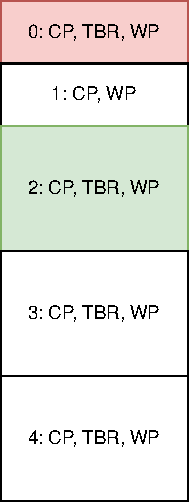
\includegraphics[width=1.0\textwidth]{block2.pdf}
		\end{column}
		\begin{column}{0.8\textwidth}

		\begin{itemize}
			\item \textbf{Table Read Protection bit}
				\begin{itemize}
					\item Block X is protected from table reads executed in other blocks
				\end{itemize}
		\end{itemize}

\begin{scriptsize}
\begin{lstlisting}[frame=single]
# setup table pointer to 0x002000
movlw 0x00
movwf TBLPTRU, A
movlw 0x20
movwf TBLPTRH, A
movlw 0x00
movwf TBLPTRL, A

# execute table read
TBLRD*

# result is in TABLAT register
buffer = TABLAT
\end{lstlisting}
\end{scriptsize}

		\end{column}
	\end{columns}

\end{frame}

\begin{frame}
	\frametitle{TBLRD Fuse}

	~\\

	\begin{center}
		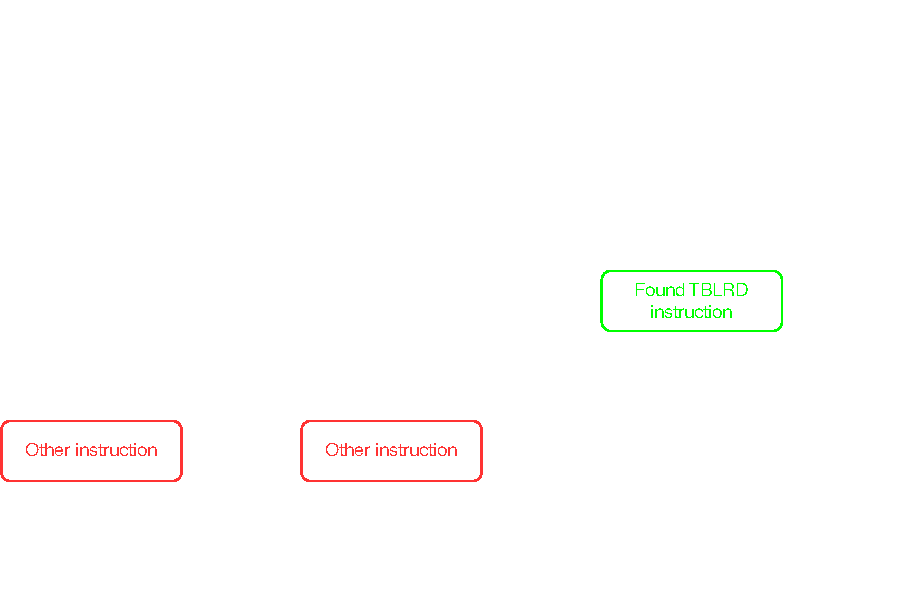
\includegraphics[width=0.9\textwidth]{flowchart-tblrd-search.pdf}
	\end{center}
\end{frame}

\begin{frame}
	\frametitle{Search Instructions Modifying PC}

	~\\

	\begin{center}
		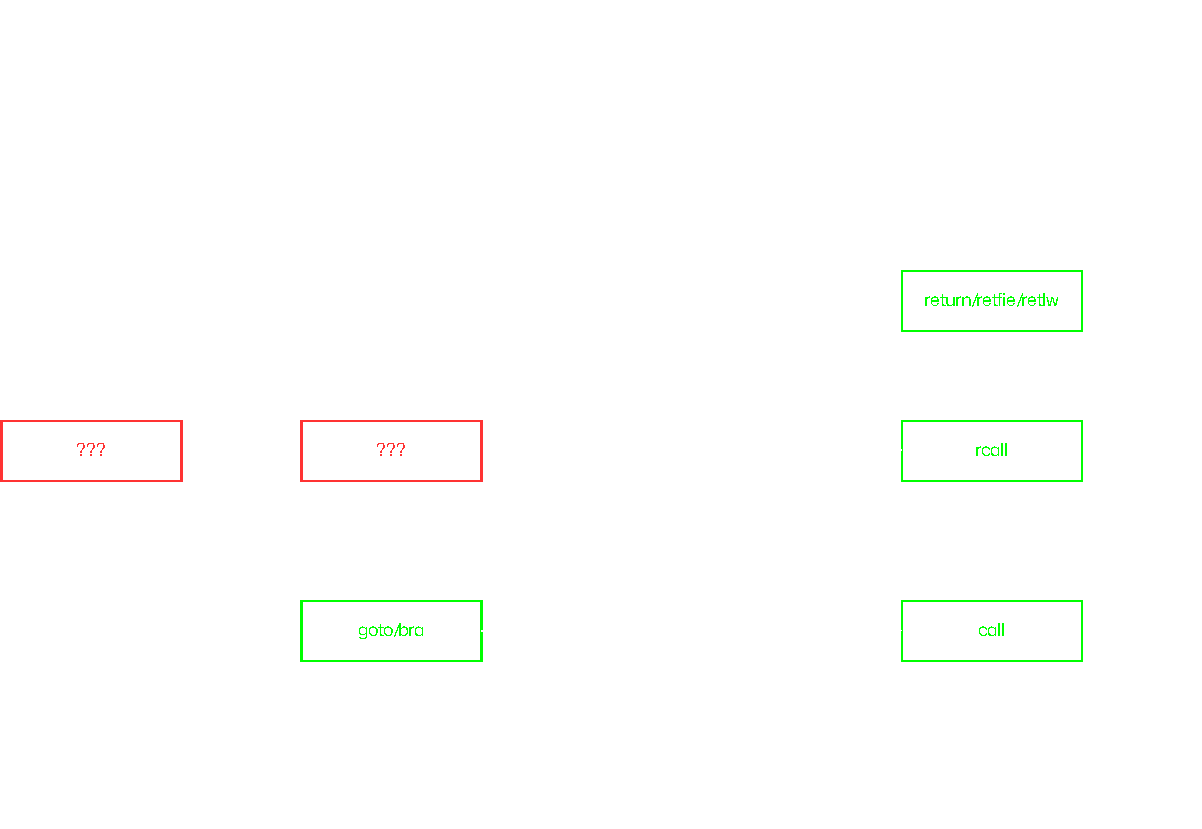
\includegraphics[width=0.9\textwidth]{flowchart-stack-search.pdf}
	\end{center}
\end{frame}

\begin{frame}[fragile]
	\frametitle{Search Remaining Instructions}

	\begin{center}
		
\includegraphics[width=0.9\textwidth]{flowchart-sram-search.pdf}
	\end{center}

\begin{scriptsize}
\begin{lstlisting}[frame=single,language=Python,commentstyle=\color{commentsColor}\textit,keywordstyle=\color{keywordsColor}\bfseries,stringstyle=\color{stringColor}]
patterns = [increment, bankincrement, const_00, const_ff, const_42]
for address in range(0x2000, 0x7fff, 1):
    for pattern in patterns:
        reset_pic()
        uart_send(address, pattern)
        result = uart_receive()
        log(address, pattern, result)
\end{lstlisting}
\end{scriptsize}
\end{frame}

\begin{frame}
	\frametitle{Instruction Recovery - Example 1}

	\begin{itemize}
		\item \texttt{Run 1: Register 0x1AF changed: 0x00 $\Rightarrow$ 0xFF}
		\item \texttt{Run 2: Register 0x1AF changed: 0xFF $\Rightarrow$ 0xFE}
		\item \texttt{Run 3: Register 0x1AF changed: 0x42 $\Rightarrow$ 0x41}
		\item \texttt{Run 4: Register 0x1AF changed: 0x11 $\Rightarrow$ 0x10}
		\item \texttt{Run 5: Register 0x1AF changed: 0xAF $\Rightarrow$ 0xAE}
	\end{itemize}
\end{frame}

\begin{frame}
	\frametitle{Instruction Recovery - Example 1}

	\begin{itemize}
		\item \texttt{Run 1: Register 0x1AF changed: 0x00 $\Rightarrow$ 0xFF}
		\item \texttt{Run 2: Register 0x1AF changed: 0xFF $\Rightarrow$ 0xFE}
		\item \texttt{Run 3: Register 0x1AF changed: 0x42 $\Rightarrow$ 0x41}
		\item \texttt{Run 4: Register 0x1AF changed: 0x11 $\Rightarrow$ 0x10}
		\item \texttt{Run 5: Register 0x1AF changed: 0xAF $\Rightarrow$ 0xAE}
		\item Probably \textbf{'DECF 0xaf, F, B'} or \textbf{'DECFSZ 0xaf, F, B'}
	\end{itemize}
\end{frame}


\begin{frame}
	\frametitle{Instruction Recovery - Example 2}

	\begin{itemize}
		\item (\texttt{Instruction is at address 0x1337DA})
		\item \texttt{Run 1: Register 0x1CC changed: 0x00 $\Rightarrow$ 0xDA}
		\item \texttt{Run 2: Register 0x1CC changed: 0xFF $\Rightarrow$ 0xDA}
		\item \texttt{Run 3: Register 0x1CC changed: 0x42 $\Rightarrow$ 0xDA}
		\item \texttt{Run 4: Register 0x1CC changed: 0x11 $\Rightarrow$ 0xDA}
		\item \texttt{Run 5: Register 0x1CC changed: 0xCC $\Rightarrow$ 0xDA}
	\end{itemize}
\end{frame}

\begin{frame}
	\frametitle{Instruction Recovery - Example 2}

	\begin{itemize}
		\item \texttt{Run 1: Register 0x1CC changed: 0x00 $\Rightarrow$ 0xDA}
		\item ...
		\item \texttt{Check instruction at 0x1337DA+1}
		\item \texttt{Run 6: Register 0x1CC changed: 0x00 $\Rightarrow$ 0xDB}
		\item \texttt{Run 7: Register 0x1CC changed: 0xFF $\Rightarrow$ 0xDB}
		\item \texttt{Run 8: Register 0x1CC changed: 0x42 $\Rightarrow$ 0xDB}
		\item \texttt{Run 9: Register 0x1CC changed: 0x11 $\Rightarrow$ 0xDB}
	\end{itemize}
\end{frame}

\begin{frame}
	\frametitle{Instruction Recovery - Example 2}

	\begin{itemize}
		\item \texttt{Check instruction at 0x1337DA}
		\item \texttt{Run 1: Register 0x1CC changed: ?? $\Rightarrow$ 0xDA}
		\item \texttt{Check instruction at 0x1337DA+1}
		\item \texttt{Run 6: Register 0x1CC changed: ?? $\Rightarrow$ 0xDB}
		\item Probably \textbf{'MOVWF 0xcc, B'}
	\end{itemize}
\end{frame}

\begin{frame}
	\frametitle{What about Block 0?}

	\begin{columns}
		\begin{column}{0.2\textwidth}
			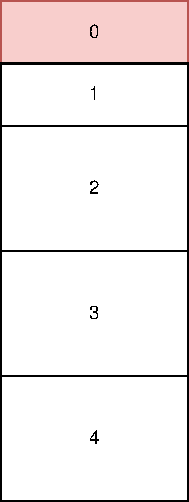
\includegraphics[width=1.0\textwidth]{block0.pdf}
		\end{column}
		\begin{column}{0.8\textwidth}
			\begin{itemize}
				\item Interrupt handler is at 0x0008 / 0x0018
					\begin{itemize}
						\item Timer IRQ does not regain code execution
						\item Except when ISR jumps into later block
					\end{itemize}
				\item It's possible to find and identify all returns
				\item It's also possible to search for traces of TBLRD
				\item Tip: use call slide instead of nop slide
					\begin{itemize}
						\item Avoids getting killed by watchdog
						\item Exact entrypoint will be available from stack
					\end{itemize}
			\end{itemize}
		\end{column}
	\end{columns}
\end{frame}

\begin{frame}
	\frametitle{Results: Lookup Table}

	\begin{columns}
		\begin{column}{0.4\textwidth}
			Found this sequence:

			\begin{itemize}
				\item ...
				\item retlw 0x7c
				\item retlw 0x77
				\item retlw 0x7b
				\item retlw 0xf2
				\item retlw 0x6b
				\item retlw 0x6f
				\item retlw 0xc5
				\item ...
			\end{itemize}
		\end{column}
		\begin{column}{0.6\textwidth}
		\end{column}
	\end{columns}
\end{frame}

\begin{frame}
	\frametitle{Results: Lookup Table}

	\begin{columns}
		\begin{column}{0.4\textwidth}
			Found this sequence:

			\begin{itemize}
				\item ...
				\item retlw 0x7c
				\item retlw 0x77
				\item retlw 0x7b
				\item retlw 0xf2
				\item retlw 0x6b
				\item retlw 0x6f
				\item retlw 0xc5
				\item ...
			\end{itemize}
		\end{column}
		\begin{column}{0.6\textwidth}
			AES S-Box:

			\begin{tabular}{|c|ccccccccc|}
				\hline
				XX  & 00 & 01 & 02 & 03 & 04 & 05 & 06 & 07 & ...\\
				\hline
				\rowcolor[RGB]{42, 42, 42}
				00  & 63 & 7c & 77 & 7b & f2 & 6b & 6f & c5 & ...\\
				10  & ca & 82 & c9 & 7d & fa & 59 & 47 & f0 & ...\\
				20  & b7 & fd & 93 & 26 & 36 & 3f & f7 & cc & ...\\
				30  & 04 & c7 & 23 & c3 & 18 & 96 & 05 & 9a & ...\\
				40  & 09 & 83 & 2c & 1a & 1b & 6e & 5a & a0 & ...\\
				50  & 53 & d1 & 00 & ed & 20 & fc & b1 & 5b & ...\\
				60  & d0 & ef & aa & fb & 43 & 4d & 33 & 85 & ...\\
				70  & 51 & a3 & 40 & 8f & 92 & 9d & 38 & f5 & ...\\
				... & ... &   &    &    &    &    &    &    & \\
				\hline
			\end{tabular}
		\end{column}
	\end{columns}
\end{frame}


\begin{frame}
	\frametitle{AES S-Box}

	\begin{center}
		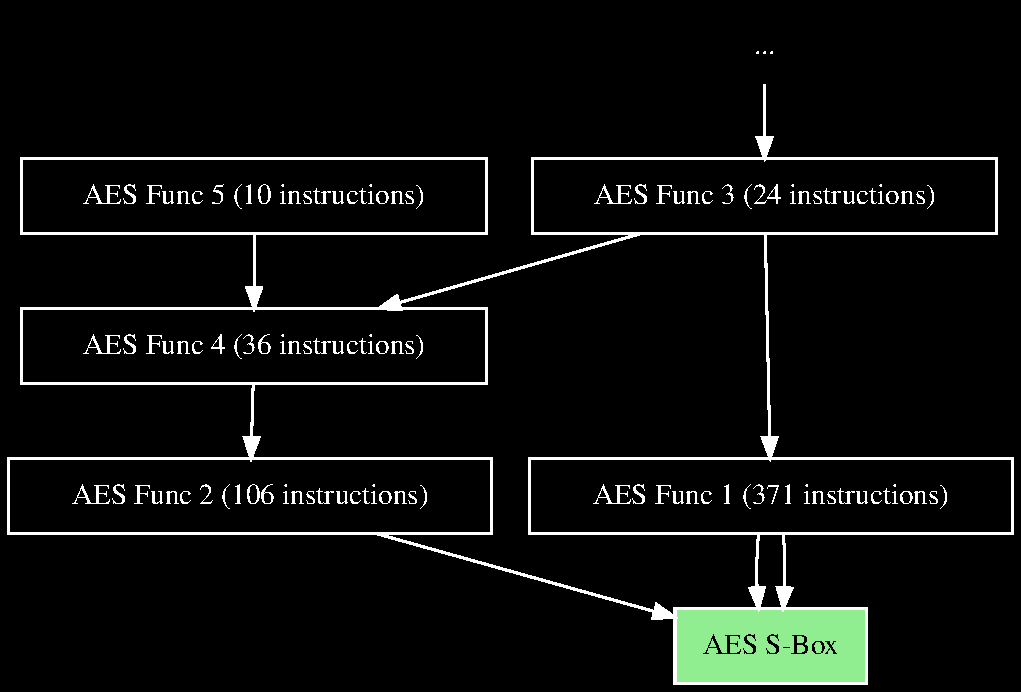
\includegraphics[width=0.8\textwidth]{small-graph-unknown.pdf}
	\end{center}
\end{frame}

\begin{frame}
	\frametitle{AES Implementations for PIC}

	\begin{columns}
		\begin{column}{0.5\textwidth}
		\end{column}
		\begin{column}{0.5\textwidth}
			\frame{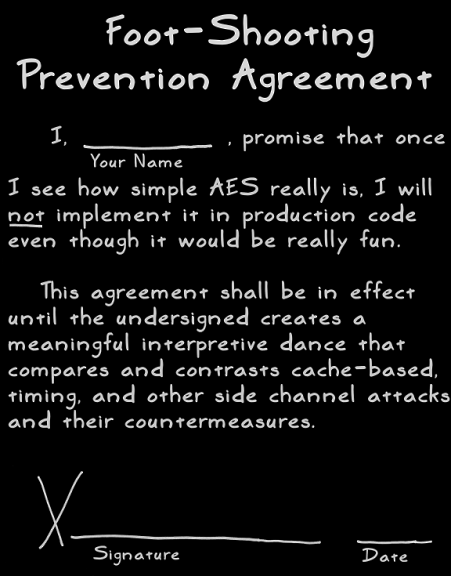
\includegraphics[height=0.85\textheight]{aes-comic.png}}\\
		\end{column}
	\end{columns}

	~\\

	\tiny{CC-BY 3.0 Jeff Moser - \url{https://www.moserware.com/2009/09/stick-figure-guide-to-advanced.html}}
\end{frame}

\begin{frame}
	\frametitle{AES Implementations for PIC}

	\begin{columns}
		\begin{column}{0.5\textwidth}
			\begin{itemize}
				\item AN953 - Data Encryption Routines for PIC18 Microcontrollers
				\item AN821 - Advanced Encryption Standard Using the PIC16XXX
			\end{itemize}
		\end{column}
		\begin{column}{0.5\textwidth}
			\frame{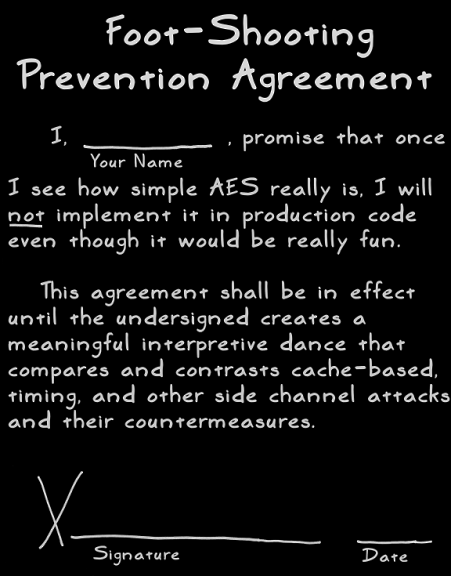
\includegraphics[height=0.85\textheight]{aes-comic.png}}\\
		\end{column}
	\end{columns}

	~\\

	\tiny{CC-BY 3.0 Jeff Moser - \url{https://www.moserware.com/2009/09/stick-figure-guide-to-advanced.html}}
\end{frame}

\begin{frame}
	\frametitle{AES Functions}

	\begin{center}
		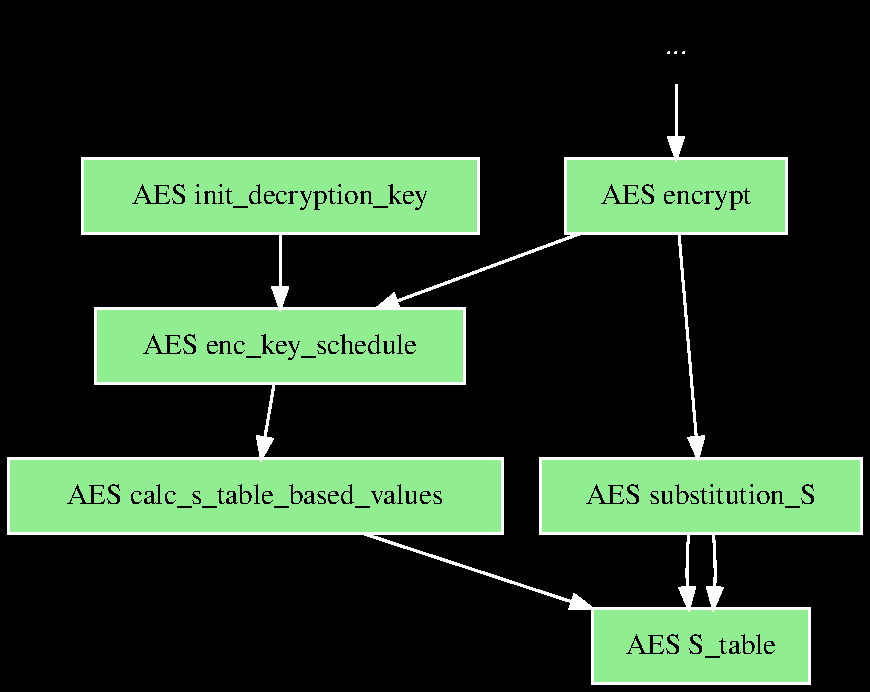
\includegraphics[height=0.9\textheight]{small-graph-named.pdf}
	\end{center}
\end{frame}

\begin{frame}
	\frametitle{UNLOCKED}

	\begin{center}
		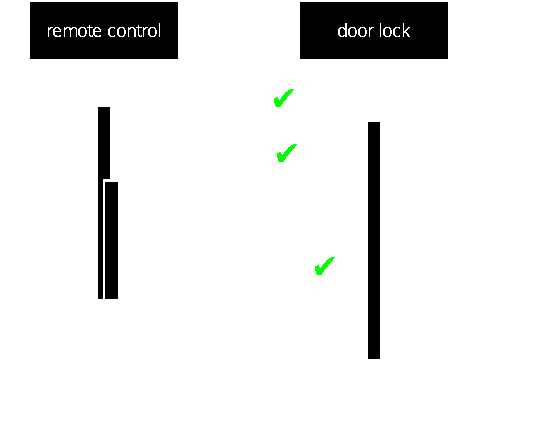
\includegraphics[width=0.6\textwidth]{communication3.pdf}
	\end{center}
\end{frame}

\begin{frame}[fragile]
	\frametitle{After Extracting the Secrets...}

	\begin{columns}
		\begin{column}{0.7\textwidth}
			\begin{small}
\begin{lstlisting}
sh> ./cff3000.py "ba:ad:c0:de:da:e5" "unlock-door1"

Remote Control Address: ba:ad:c0:de:da:e5
Command Byte: 11

Sending control requests...
  ab ba ad c0 de da e5 11 00 00 00 00 00 00 00 00
Receiving challenge...
  ab 54 25 f3 12 52 a1 11 6e 95 a2 69 cd b3 00 02
Sending encrypted response...
  4d db 88 48 33 c6 33 ec e6 7f 5b 26 51 c7 38 a5
\end{lstlisting}
			\end{small}
		\end{column}
		\begin{column}{0.3\textwidth}
			\begin{center}
				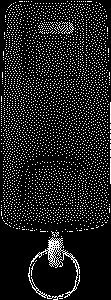
\includegraphics[height=0.8\textheight]{cff3000-dithered.png}
			\end{center}
		\end{column}
	\end{columns}
\end{frame}

\begin{frame}
	\frametitle{Responsible Disclosure}

	\begin{itemize}
		\item \texttt{rC3 ~ 2021} - Found AES S-Box
		\item \texttt{10.01.2022} - Full door lock access
		\item \texttt{31.01.2022} - Ask disclosure@ccc.de for prior experience with Abus
		\item \texttt{08.02.2022} - Report to CERT-BUND
		\item \texttt{22.07.2022} - MCH2022
	\end{itemize}
\end{frame}

\begin{frame}
	\frametitle{10.08.2022 - Product Warning}

	\begin{center}
		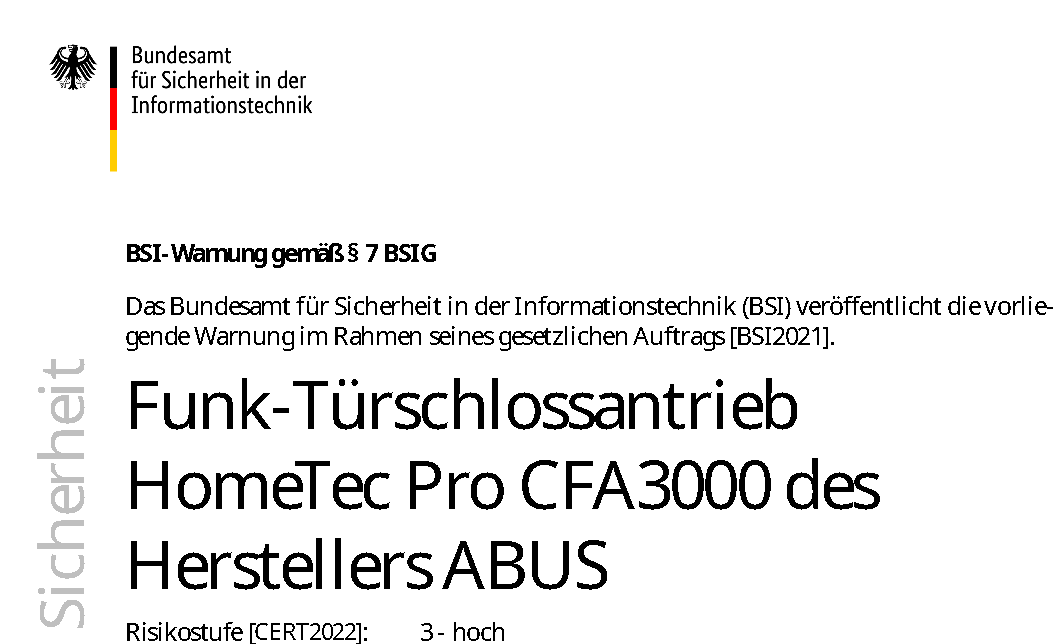
\includegraphics[height=0.85\textheight]{BSI-Abus-Warnung.pdf}
	\end{center}
\end{frame}

\begin{frame}
	\frametitle{How we handled it}

	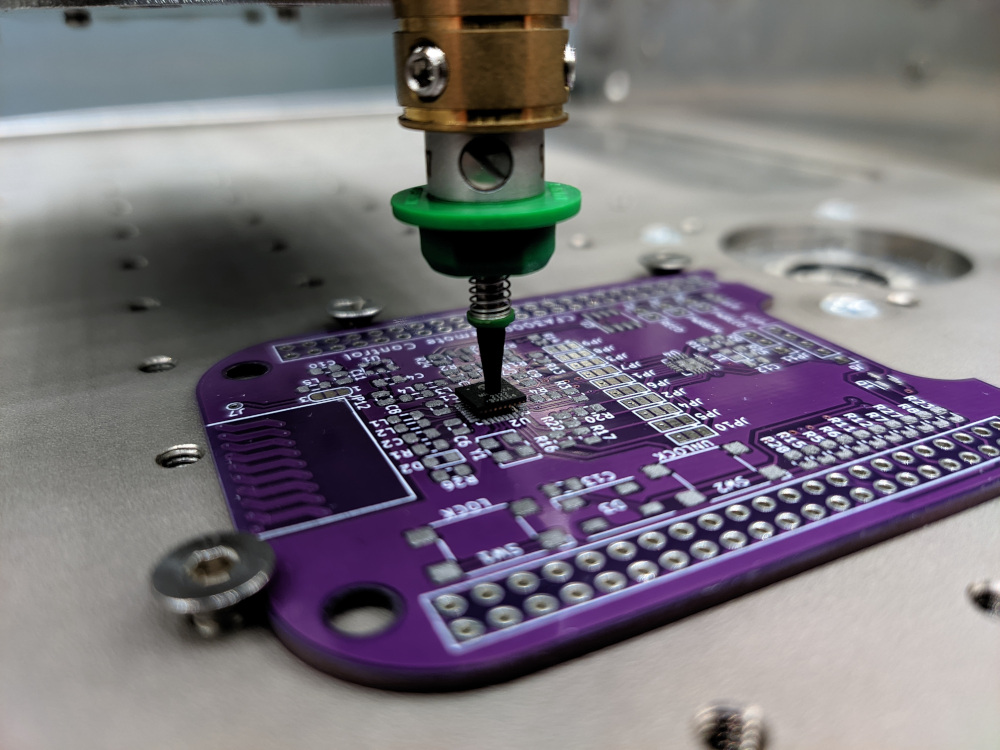
\includegraphics[height=0.55\textheight]{MRF89XA-BBB-Cape-1.jpg}
	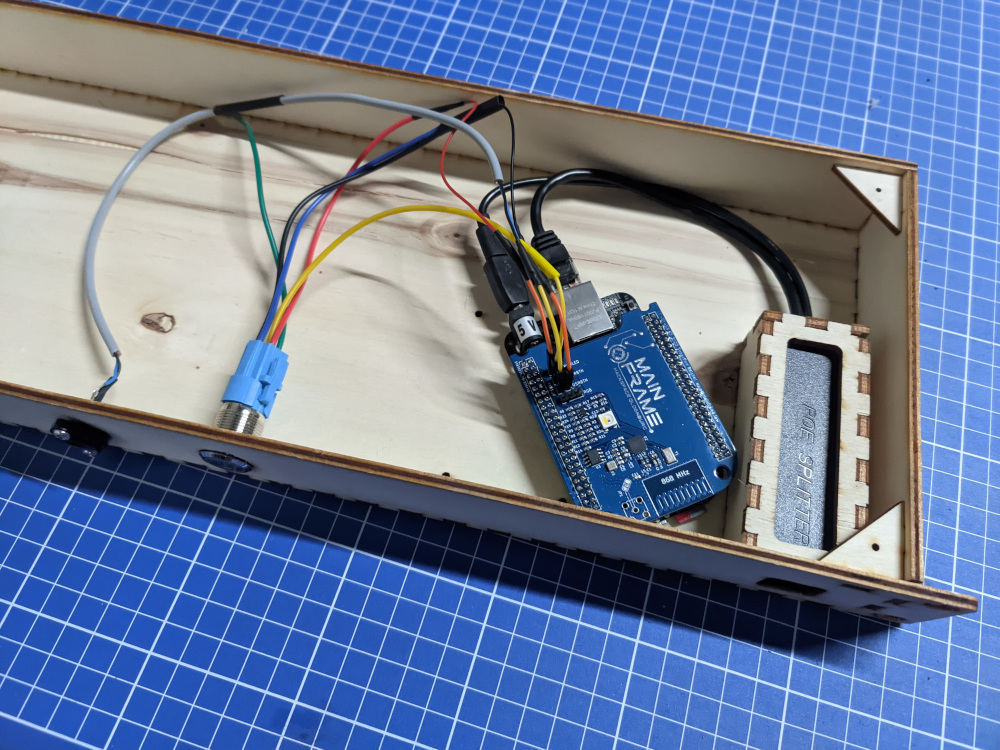
\includegraphics[height=0.55\textheight]{MRF89XA-BBB-Cape-3.jpg}

	\begin{itemize}
		\item Sorry, no open FW
	\end{itemize}
\end{frame}

\begin{frame}
	\frametitle{Questions?}

	\large

	\begin{itemize}
		\item sre@mainframe.io
		\item EF66-0D07-463F-8B72-6A79-5413-D8EE-D7F3-C83B-FA9A
	\end{itemize}
\end{frame}

\begin{frame}
	\frametitle{Links}

	\begin{itemize}
		\item Gnuradio files \url{https://github.com/sre/mrf89xa-gnuradio}
		\item KiCAD files: \url{https://github.com/sre/bbb-mrf89xa-cape}
		\item PIC Programmer Software: \url{https://github.com/sre/picberry}
		\item Datasheets
			\begin{itemize}
				\item \url{https://www.microchip.com/en-us/product/MRF89XA}
				\item \url{https://www.microchip.com/en-us/product/PIC16F1829}
				\item \url{https://www.microchip.com/en-us/product/PIC18LF45K80}
			\end{itemize}
		\item BSI Product Warning: \url{https://www.bsi.bund.de/SharedDocs/Downloads/DE/BSI/Publikationen/Warnungen-nach-P7_BSIG/Archiv/2022/BSI_W-005-220810.pdf?__blob=publicationFile&v=16}
	\end{itemize}
\end{frame}

%------------------------------------------------------------------------

\begin{frame}
	\frametitle{Bonus: SDR Transceiver}

	\begin{center}
		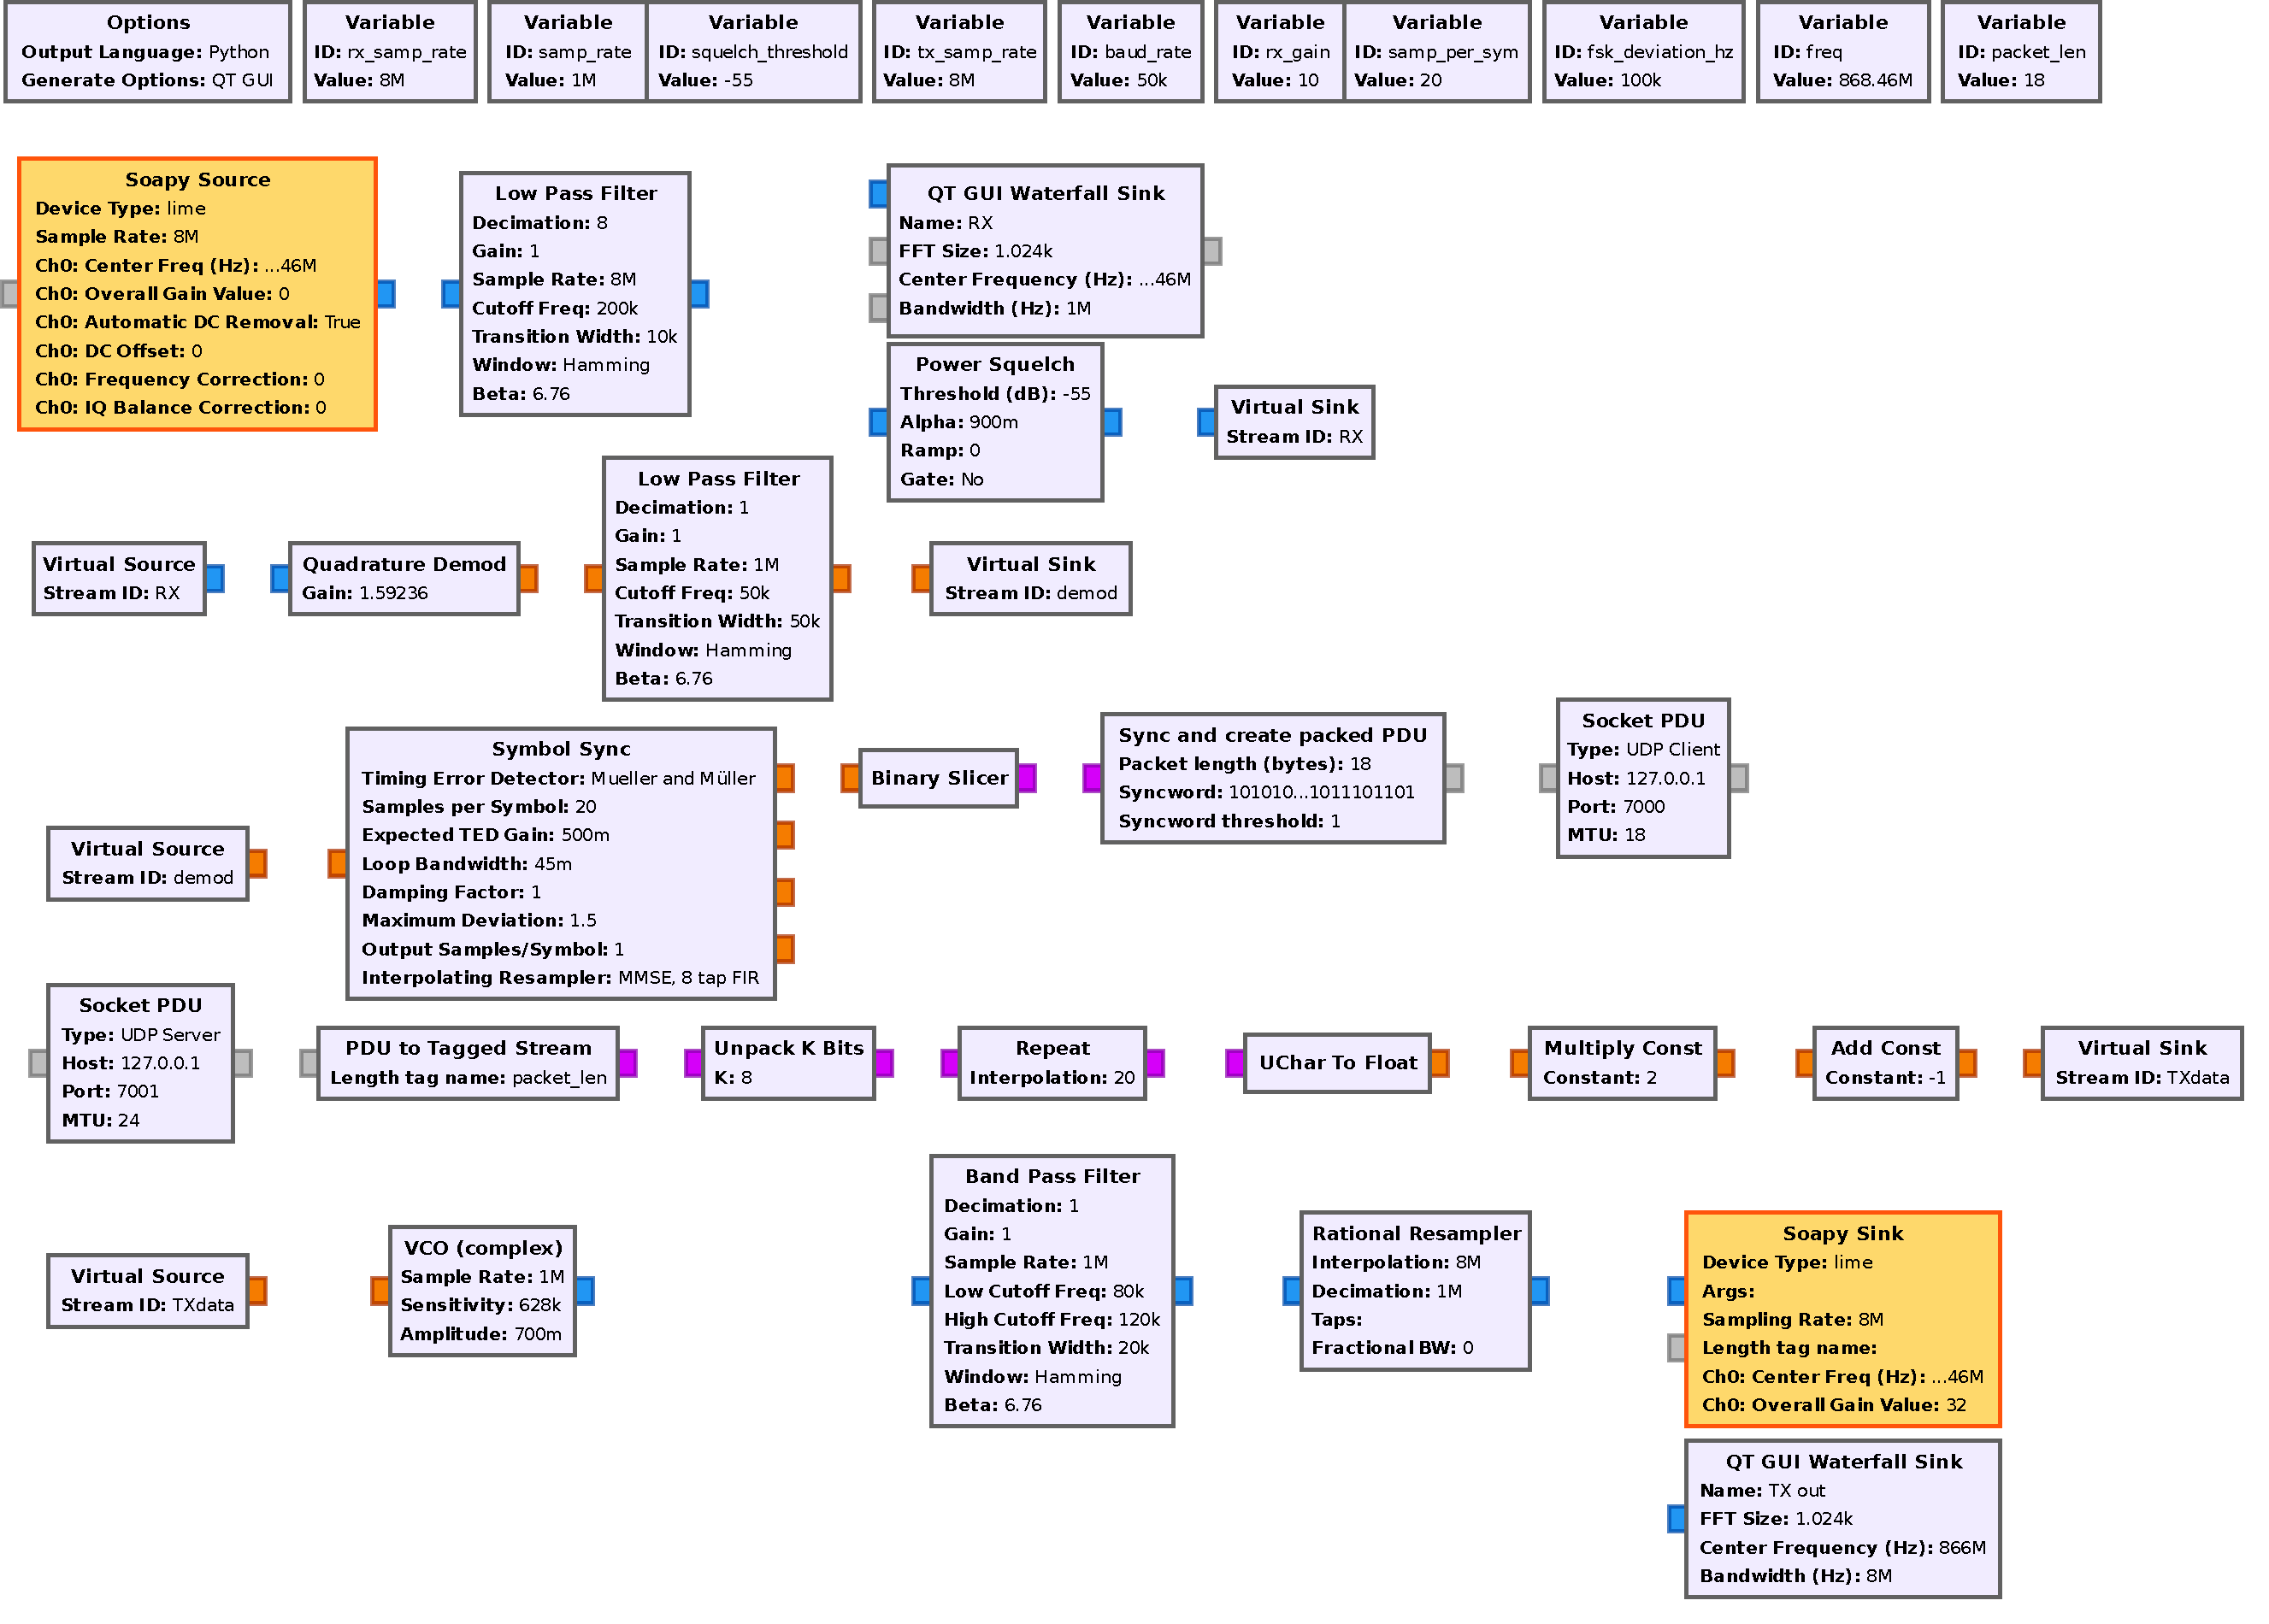
\includegraphics[height=0.9\textheight]{full-gnuradio-pipeline-dark.pdf}
	\end{center}
\end{frame}

\begin{frame}[fragile]
	\frametitle{Bonus: MRF89XA dewhitening}

\begin{scriptsize}
\begin{lstlisting}[frame=single,showstringspaces=false,language=Python,commentstyle=\color{commentsColor}\textit,keywordstyle=\color{keywordsColor}\bfseries,stringstyle=\color{stringColor}]
#!/usr/bin/python3
import socket

lfsrdata = [0xff, 0x87, 0xb8, 0x59, 0xb7, 0xa1, 0xcc, 0x24,
            0x57, 0x5e, 0x4b, 0x9c, 0x0e, 0xe9, 0xea, 0x50,
            0x2a, 0xbe]

def dewhite(msg):
    return [pair[0] ^ pair[1] for pair in zip(msg, lfsrdata)]

def printmsg(rawmsg):
    msg = dewhite(rawmsg)
    print(' '.join(["{:02x}".format(x) for x in msg]))

sock = socket.socket(socket.AF_INET, socket.SOCK_DGRAM)
sock.bind(("127.0.0.1", 1337))

while True:
    printmsg(sock.recv(18))
\end{lstlisting}
\end{scriptsize}
\end{frame}

\begin{frame}[fragile]
	\frametitle{Bonus: MRF89XA CRC calculation}

\begin{scriptsize}
\begin{lstlisting}[frame=single,showstringspaces=false,language=Python,commentstyle=\color{commentsColor}\textit,keywordstyle=\color{keywordsColor}\bfseries,stringstyle=\color{stringColor}]
def crc16_ccitt(data, crc = 0x1D0F):
    msb = crc >> 8
    lsb = crc & 255
    for c in data:
        x = c ^ msb
        x ^= (x >> 4)
        msb = (lsb ^ (x >> 3) ^ (x << 4)) & 0xff
        lsb = (x ^ (x << 5)) & 0xff
    crc = (msb << 8) + lsb
    # MRF89XA uses negated CRC
    return ~crc & 0xffff

def printmsg(rawmsg):
    msg = dewhite(rawmsg)
    crc = msg[16] << 8 | msg[17]
    msg = msg[0:16]
    crc2 = crc16_ccitt(msg)
    text = ' '.join(["{:02x}".format(x) for x in msg[0:16]])
    if crc == crc2:
        print(text + " OK")
    else:
        print("FAIL")
\end{lstlisting}
\end{scriptsize}
\end{frame}

\begin{frame}[fragile]
	\frametitle{Bonus: ASM Code for the Timer / goto logic}

\begin{tiny}
\begin{lstlisting}[frame=single]
# 0. implement IRQ handler, which dumps TABLAT via UART
# 1. init PIC (clear watchdog, setup clocks, setup timer, setup UART)
# 2. read address that should be analyzed via UART into register 0x00-0x02
# 3. 'call' that address like this:

# copy UART provided address into TBLRD address register
movff 0x00, TBLPTRU
movff 0x01, TBLPTRH
movff 0x02, TBLPTRL

# trigger timer irq in 0xff-0xf5+1 = 11 instructions
movlw 0xF5
movwf TMR0L, A
bsf T0CON, 7

# prepare program counter latch register
movff 0x00, PCLATU
movff 0x01, PCLATH

# put return address on stack
push
movf TOSL, W, A
addlw 0x0C
movwf TOSL, A

# jump to UART provided address
movf 0x02, W, A
movwf PCL, A

# only reached when target address modifies timer behaviour
\end{lstlisting}
\end{tiny}
\end{frame}

\begin{frame}[fragile]
	\frametitle{Bonus: ASM Code IRQ handler}

\begin{tiny}
	\begin{columns}
		\begin{column}{0.5\textwidth}
\begin{lstlisting}[frame=single]
setup_uart:
    # enable UART module (UART1MD = 0)
    banksel PMD0
    bcf PMD0, 1, B
    # RC6 = TX1 = pin 1 = output
    bcf TRISC, 6, A
    # RC7 = RX1 = pin 44 = input
    bcf TRISC, 7, A
    # TXSTA1 = 0x00
    clrf TXSTA1, A
    # RCSTA1 = 0x90
    movlw 0x90
    movwf RCSTA1, A
    # BAUDCON1 = 0x00
    clrf BAUDCON1, A
    # PIR1 = 0x00
    clrf PIR1, A
    # PIE1 = 0x00
    clrf PIE1, A
    # SPBRGH1 = 0
    clrf SPBRGH1, A
    # SPBRG1 = 25
    movlw 0x19
    movwf SPBRG1, A
    ret
\end{lstlisting}
		\end{column}
		\begin{column}{0.5\textwidth}
\begin{lstlisting}[frame=single]
regdump:
    call print_register_tosh;
    call print_register_tosl;
    pop
    call print_register_tosh;
    call print_register_tosl;
    ...
    call print_register_5f;
    call print_register_5e;
    ...
    ret
\end{lstlisting}
\begin{lstlisting}[frame=single]
__irq_handler:
    # disable timer
    bcf T0CON, 7
    # save special regs, so that they can be dumped later
    movff WREG, 0x05F
    movff STATUS, 0x05E
    movff BSR, 0x05D
    # clear watchdog
    clrwdt
    # re-setup UART
    call uart_setup
    # dump interesting registers
    call regdump
    # wait for system reset
hangup_irq_handler:
    clrwdt
    bra hangup_irq_handler
\end{lstlisting}
		\end{column}
	\end{columns}
\end{tiny}
\end{frame}

\begin{frame}
	\frametitle{Bonus: CFF3000 PIC16F1829 Pinout}

	\begin{center}
		\begin{tabular}{|c|c|c||c|c|c|}
			\hline
			Pin & Name & Description & Pin & Name & Description\\
			\hline
			 1 & RA3 & Lock        & 11 & RC2 & RF CSDAT\\
			 2 & RC5 & Charge Pump & 12 & RC1 & RF CSCON\\
			 3 & RC4 & VDD enable  & 13 & RC0 & RF TEST8\\
			 4 & RC3 & RF PLOCK    & 14 & RA2 & UNLOCK\\
			 5 & RC6 & RF DATA     & 15 & RA1 & ICSP CLK\\
			 6 & RC7 & RF SDI      & 16 & RA0 & ICSP DAT\\
			 7 & RB7 & RF IRQ1     & 17 & VSS & VSS\\
			 8 & RB6 & RF SCK      & 18 & VDD & VDD\\
			 9 & RB5 & RF IRQ0     & 19 & RA5 & LED RED\\
			10 & RB4 & RF SDO      & 20 & RA4 & LED GREEN\\
			\hline
		\end{tabular}
	\end{center}
\end{frame}

\begin{frame}
	\frametitle{Bonus: CFA3000 PIC18LF45K80 Pinout}

	\begin{scriptsize}
	\begin{tabular}{|c|c|c||c|c|c||c|c|c|}
		\hline
		Pin & Name & Description & Pin & Name & Description & Pin & Name & Description\\
		\hline
		 1 & RC7 & Button Shield  & 16 & RB6 & Reed B         & 31 & RA6 & Voltage Regulator\\
		 2 & RD4 & Motor A Pos    & 17 & RB7 & Volt. Div. Out & 32 & RC0 & RF PLOCK\\
		 3 & RD5 & Motor A Neg    & 18 & RE3 & MCLR           & 33 & N/C & ---\\
		 4 & RD6 & Motor B Neg    & 19 & RA0 & Button Down    & 34 & N/C & ---\\
		 5 & RD7 & Motor B Pos    & 20 & RA1 & Button Up      & 35 & RC1 & RF DATA\\
		 6 & VSS & VSS            & 21 & RA2 & Button Lock    & 36 & RC2 & RF CSDAT\\
		 7 & VDD & VDD            & 22 & RA3 & Button Unlock  & 37 & RC3 & RF SCK\\
		 8 & RB0 & RF IRQ0        & 23 & VCAP & VDDCORE       & 38 & RD0 & LED Right\\
		 9 & RB1 & RF IRQ1        & 24 & RA5 & ???            & 39 & RD1 & LED Left\\
		10 & RB2 & VBACKEMF       & 25 & RE0 & Voltage Meas.  & 40 & RD2 & LED Right\\
		11 & RB3 & VBACKEMF       & 26 & RE1 & VShunt         & 41 & RD3 & LED Left\\
		12 & N/C & ---            & 27 & RE2 & RF RESET       & 42 & RC4 & RF SDO\\
		13 & N/C & ---            & 28 & VDD & VDD            & 43 & RC5 & RF SDI\\
		14 & RB4 & Reed A         & 29 & VSS & VSS            & 44 & RC6 & RF CSCON\\
		15 & RB5 & Buzzer (4 kHz) & 30 & RA7 & BAT SER/PAR    & & &\\
		\hline
	\end{tabular}
	\end{scriptsize}
\end{frame}

\end{document}
